%!TEX program = xelatex

% 纸张模式:护眼模式-geye 朦胧模式-hazy
% 纸张尺寸:pad kindle pc normal screen

\documentclass[cn, hazy, blue, normal, 12pt]{elegantnote}

\title{数字信号处理笔记}
\author{Xiaohei}
\institute{Created by Elegant\LaTeX{}}
\version{1.4}
\date{\zhtoday}

\usepackage{tikz}
\usepackage{amssymb}
\usepackage{pgfplots}
\usepackage{bookmark}
\usepackage{multirow}
\usepackage{tabularx}

\begin{document}

\maketitle

\section{离散时间信号与系统}

\subsection{离散时间信号——序列}

\subsubsection{离散时间信号——序列}

一般用$x(n)$表示离散时间信号(序列),$x(n)$可以看成是对模拟信号$x(n)$的等间隔抽样,即

\begin{equation}
        x(n)=\left.x_a(t)\right|_{t=nT}=x_a(nT)
\end{equation}

序列的表示方法:函数表示法、数列表示法、图形表示法。

$$x_1(n)=2n(0.9)^n, \quad x_2(n)=\{1, \underline{1}, 4, 5, 1, 4\}$$

\begin{center}
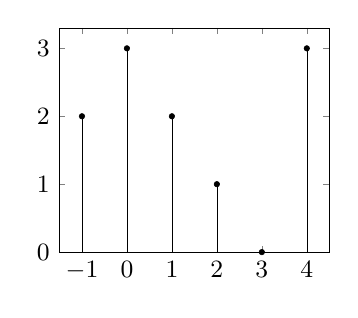
\begin{tikzpicture}[scale=0.5]
\tikzstyle{every node}=[font=\small,scale=2]
\begin{axis}[ymin=0]
    \addplot[ycomb, mark=*] coordinates 
    {(-1, 2) (0, 3) (1, 2) (2, 1) (3, 0) (4, 3)};
\end{axis}
\end{tikzpicture}
\end{center}

\subsubsection{序列的运算}

序列的运算:移位、翻褶、和、积、累加、差分、时间尺度变换、卷积和。

\textbf{移位}

\begin{equation}
        y(n)=x(n-n_0)
\end{equation}

当$n_0>0$时,序列右移(延迟);当$n_0<0$时,序列左移(超前)。

计算方法:用$n-n_0$代替序列表达式中的每个$n$,然后化简,即可求$x(n-n_0)$。

\textbf{翻褶}

\begin{equation}
        y(n)=x(-n)
\end{equation}

计算方法:用$-n$代替序列表达式中的每个$n$,然后化简,即可求$x(-n)$。

\textbf{和}

两序列的和是指同序号($n$相同)的序列值逐项对应相加而构成的一个新的序列,表示为

\begin{equation}
        z(n)=x(n)+y(n)
\end{equation}

计算方法:同区间的序列表达式先相加,其它序列值逐项对应相加。注意同时刻对齐。 

\textbf{积}

两序列的积是指同序号($n$相同)的序列值逐项对应相乘而构成的一个新的序列,表示为

\begin{equation}
        z(n)=x(n)\cdot y(n)
\end{equation}

计算方法:同区间的序列表达式先相乘,其它序列值逐项对应相乘。注意同时刻对齐。

\textbf{累加}

设某序列为$x(n)$,则它的累加序列定义为

\begin{equation}
        y(n)=\sum_{k=-\infty}^n x(k)
\end{equation}

\textbf{差分}

前向差分:

\begin{equation}
        \Delta x(n)=x(n+1)-x(n)
\end{equation}

后向差分:

\begin{equation}
        \nabla x(n)=x(n)-x(n-1)
\end{equation}

这里的$x(n)$、$x(n+1)$、$x(n-1)$是同一个序列中的采样值。前向差分是下一个采样值减去当前采样值,不能实时实现;后向差分是当前采样值减去过去一个采样值,可实时实现。 

\textbf{时间尺度变换}

设某序列为$x(n)$,其时间尺度变换序列为

\begin{equation}
        x(mn) \text{ or } x(n/m)
\end{equation}

其中$m$为正整数。$x(mn)$称为抽取序列,而$x(n/m)$则称为插值序列。

变换后的序列值同原序列相比,只有$n=0$处的序列值的位置不变。序列插值在原序列的两个序列值之间插入$m-1$个值,一般为$0$。也可定义其它的值。序列抽取是非线性运算,运算不可逆。

\textbf{卷积和}

卷积和亦称线性卷积。它是求离散线性移不变系统零状态相应的主要方法。设两序列为$x(n)$和$h(n)$,定义这两个序列的卷积和为

\begin{equation}
        y(n)=\sum_{m=-\infty}^{\infty}{x(m)h(n-m)}=x(n)\ast h(n)
\end{equation}

计算方法:翻褶、移位、相乘、相加。

卷积和有交换律。

\subsubsection{几种常用典型序列}

\textbf{单位抽样序列}

\begin{equation}
        \delta(n)= \left\{
        \begin{array}{rl}
        1 & \text{if } n = 0,\\
        0 & \text{if } n \neq 0.
        \end{array}
        \right.
\end{equation}

\begin{center}
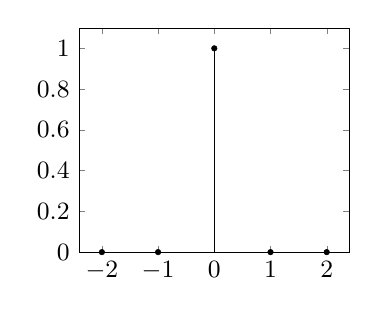
\begin{tikzpicture}[scale=0.5]
\tikzstyle{every node}=[font=\small,scale=2]
\begin{axis}[ymin=0]
    \addplot[ycomb, mark=*] coordinates 
    {(-2, 0) (-1, 0) (0, 1) (1, 0) (2, 0)};
\end{axis}
\end{tikzpicture}
\end{center}

\textbf{单位阶跃序列}

\begin{equation}
        u(n)= \left\{
        \begin{array}{rl}
        1 & \text{if } n \geq 0,\\
        0 & \text{if } n \leq 0.
        \end{array}
        \right.
\end{equation}

\begin{center}
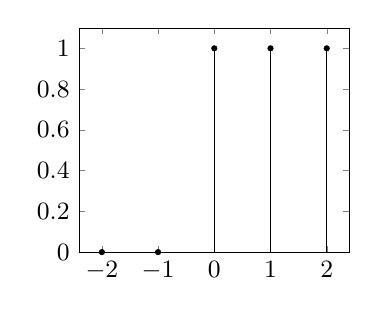
\begin{tikzpicture}[scale=0.5]
\tikzstyle{every node}=[font=\small,scale=2]
\begin{axis}[ymin=0]
    \addplot[ycomb, mark=*] coordinates 
    {(-2, 0) (-1, 0) (0, 1) (1, 1) (2, 1)};
\end{axis}
\end{tikzpicture}
\end{center}

\textbf{$\delta(n)$与$u(n)$之间的关系}

$$\delta(n)=u(n)-u(n-1), \quad u(n)=\sum_{k=0}^{\infty}{\delta(n-k)}$$

\textbf{矩形序列}

\begin{equation}
    R_N(n)= \left\{
    \begin{array}{rl}
    1 & \text{if } 0 \leq n \leq N-1,\\
    0 & \text{others}.
    \end{array}
    \right.
\end{equation}

\begin{center}
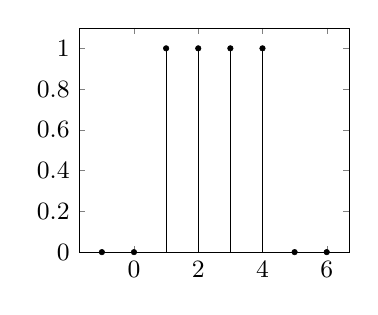
\begin{tikzpicture}[scale=0.5]
\tikzstyle{every node}=[font=\small,scale=2]
\begin{axis}[ymin=0]
    \addplot[ycomb, mark=*] coordinates 
    {(-1, 0) (0, 0) (1, 1) (2, 1) (3, 1) (4, 1) (5, 0) (6, 0)};
\end{axis}
\end{tikzpicture}
\end{center}

\textbf{实指数序列}

\begin{equation}
        x(n)=a^{n}u(n),a\in\mathbb{R}
\end{equation}

\begin{center}
\begin{minipage}[t]{0.3\linewidth}
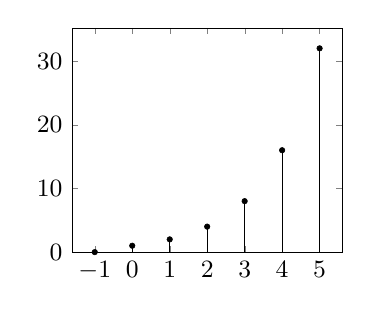
\begin{tikzpicture}[scale=0.5]
\tikzstyle{every node}=[font=\small,scale=2]
\begin{axis}[ymin=0]
    \addplot[ycomb, mark=*] coordinates 
    {(-1, 0) (0, 1) (1, 2) (2, 4) (3, 8) (4, 16) (5, 32)};
\end{axis}
\end{tikzpicture}
\end{minipage}
\begin{minipage}[t]{0.3\linewidth}
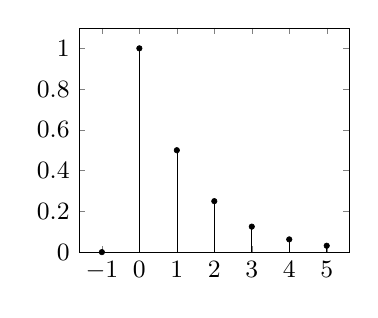
\begin{tikzpicture}[scale=0.5]
\tikzstyle{every node}=[font=\small,scale=2]
\begin{axis}[ymin=0]
    \addplot[ycomb, mark=*] coordinates 
    {(-1, 0) (0, 1) (1, 0.5) (2, 0.25) (3, 0.125) (4, 0.0625) (5, 0.03125)};
\end{axis}
\end{tikzpicture}
\end{minipage}
\begin{minipage}[t]{0.3\linewidth}
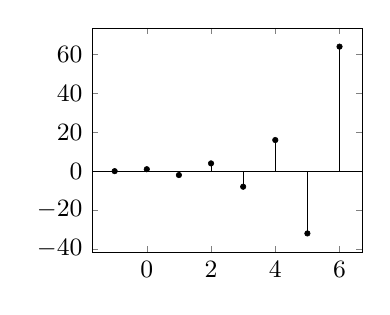
\begin{tikzpicture}[scale=0.5]
\tikzstyle{every node}=[font=\small,scale=2]
\begin{axis}
    \addplot[ycomb, mark=*] coordinates 
    {(-1, 0) (0, 1) (1, -2) (2, 4) (3, -8) (4, 16) (5, -32) (6, 64)};
    \addplot[black, sharp plot, update limits=false] 
	coordinates {(-2, 0) (7, 0)};
\end{axis}
\end{tikzpicture}
\end{minipage}
\end{center}

\textbf{正弦序列}

\begin{equation}
        x(n)=A\sin(n\omega_0+\phi)
\end{equation}

\begin{center}
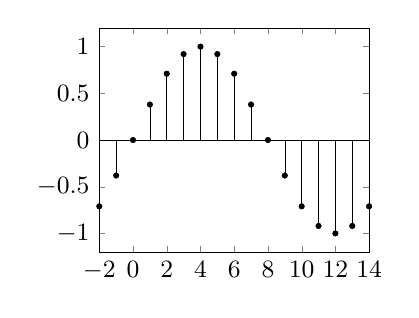
\begin{tikzpicture}[scale=0.5]
\tikzstyle{every node}=[font=\small,scale=2]
\begin{axis}[xmin=-2, xmax=14]
    \addplot[ycomb, mark=*] coordinates 
    {(-2, -0.71) (-1, -0.38) (0, 0) (1, 0.38) (2, 0.71) (3, 0.92) (4, 1) (5, 0.92) (6, 0.71) (7, 0.38) (8, 0) (9, -0.38) (10, -0.71) (11, -0.92) (12, -1) (13, -0.92) (14, -0.71)};
    \addplot[black, sharp plot, update limits=false] 
	coordinates {(-2, 0) (14, 0)};
\end{axis}
\end{tikzpicture}
\end{center}

\textbf{复指数序列}

\begin{equation}
        x(n)={\rm{e}}^{(\sigma+{\rm{j}}\omega_0)n}
\end{equation}

复指数序列是实部和虚部都是指数型的正弦序列。复指数序列可以表示任意的序列。

\subsubsection{序列的周期性}

如果存在一个最小的正整数$N$,满足$x(n)=x(n+N)$,则序列$x(n)$为周期性序列,$N$为最小周期。

对于$x(n)=A\sin(n\omega_0+\phi)$:

\begin{quote}
\begin{enumerate}
    \item 若$\dfrac{2\pi}{\omega_0}=\dfrac{N}{M}, M,N\in\mathbb{N+}$,且$N, M$互素,则正弦序列周期为$N$。
    \item 若$\dfrac{2\pi}{\omega_0}$为无理数,则正弦序列不是周期性序列。
\end{enumerate}
\end{quote}

周期性序列$x(n)$的周期为$N$,若$x(n)$由模拟的正弦信号采样而来,则表示每$M$个模拟周期内采样了$N$个序列值。

设采样周期为$T$,则数字频率与模拟频率之间的关系:$\omega_0=\Omega_0T$。数字频率表示模拟信号在一个采样周期内变化的角度或模拟信号的频率对采样频率归一化的$2\pi$倍。

\subsubsection{序列的分解}

用单位抽样序列来表示任意序列$x(n)$

\begin{equation}
        x(n)=\sum_{m=-\infty}^{\infty}{x(m)\delta(n-m)}
\end{equation}

\subsubsection{序列的能量}

序列$x(n)$的能量$E$定义为序列各抽样值的平方和,即

\begin{equation}
        E=\sum_{n=-\infty}^{\infty}{|x(n)|^2}
\end{equation}

\subsection{线性移不变系统}

系统可定义为将输入序列$x(n)$映射成输出序列$y(n)$的唯一变换运算,并用$T[]$表示,即

\begin{equation}
        y(n)=T[x(n)]
\end{equation}

若系统满足可加性与比例性,则称此系统为离散时间线性系统。

\begin{equation}
        y(n)=T[ax_1(n)+bx_2(n)]=aT[x_1(n)]+bT[x_2(n)]=ay_1(n)+by_2(n)
\end{equation}

若系统输入移动$n_0$位,其输出也移动$n_0$位,且幅值保持不变,则称此系统为移不变系统。

\begin{equation}
        y(n-n_0)=T[x(n-n_0)]
\end{equation}

\subsection{常系数线性差分方程}

在离散线性移不变系统中,常用常系数线性差分方程表示输入输出关系

\begin{equation}
        \sum_{k=0}^{N}{a_k y(n-k)}=\sum_{m=0}^{M}{b_m x(n-m)}
\end{equation}

或

\begin{equation}
        y(n)=\sum_{m=0}^{M}{b_m x(n-m)}-\sum_{k=1}^{N}{a_k y(n-k)}
\end{equation}

\begin{quote}
\begin{enumerate}
    \item 常系数:$a_k, b_m$均是常数(不含$n$)。
    \item 阶数:输出变量$y(n)$中$n$的最大序号与最小序号之差。
    \item 线性:$y(n-k)$,$x(n-m)$各项只有一次幂,不含它们的乘积项。
\end{enumerate}
\end{quote}

用迭代法求$h(n)$:当$x(n)=\delta(n)$时,$y(n)=h(n)$。

一个常系数线性差分方程并不一定代表因果系统,也不一定表示线性移不变系统。这些都由边界条件(初始状态)所决定。假定系统的初始状态为$0$,常系数线性差分方程就代表线性移不变系统,且多为因果系统。

\subsection{连续时间信号的抽样}

抽样是利用周期性脉冲系列$p(t)$,从连续信号$x_a(t)$中抽取一系列的离散值$\hat{x}_a(t)$,即为抽样信号(序列)。

$p(t)\rightarrow\delta_T(t)$,$\delta_T(t)$是以$T$为周期的周期冲激序列,表示为

\begin{equation}
        \delta_T(t)=\sum_{m=-\infty}^{\infty}{\delta(t-mT)}
\end{equation}

\textbf{理想抽样}:$\hat{x}_a(t)=\sum\limits_{m=-\infty}^{\infty}{x_a(mT)\delta(t-mT)}$。

理想抽样后的频谱是对原频谱的周期延拓。若原连续信号最高频率为$\Omega_h$,采样率为$\Omega_s$,则抽样后$k=0$时,为原频谱的$1/T$,$k\neq 0$时,为原频谱的$1/T$右移$k\Omega_s$单位。

当$\Omega_h>\Omega_s/2$时,频谱会发生重叠。$\Omega_s/2$称作折叠频率。当$\Omega_h<\Omega_s/2$时,频谱不会发生混叠,才可以恢复原信号。为了避免混叠,一般在抽样器前加一个保护性的前置低通滤波器,称为防混叠滤波器,其截止频率为$\Omega_s/2$,以便滤除掉高于$\Omega_s/2$的频率分量。

低通滤波器的冲激响应

\begin{equation}
        h(t)=\text{Sa}\left(\dfrac{\pi}{T}t\right)
\end{equation}

低通滤波器的输出

\begin{equation}
        y_a(t)=\int_{-\infty}^{\infty}{\hat{x}_a(\tau)h(t-\tau)\text{d}\tau}=\sum\limits_{m=-\infty}^{\infty}{x_a(mT)\text{Sa}[\dfrac{\pi}{T}(t-mT)]}
\end{equation}

其中$x_a(mT)$是抽样序列,$\text{Sa}[\dfrac{\pi}{T}(t-mT)]$称为内插函数,在抽样点$mT$上,其值为$1$;其余抽样点上,其值为$0$。在抽样点上,信号值不变;抽样点之间的信号则由各抽样函数波形的延伸叠加而成。    


\textbf{实际抽样}:$\hat{x}_a(t)=x_a(t)\cdot P_{\tau}(t)$。

实际抽样中,采样定理仍有效;$\hat{x}_a(\text{j}\Omega)$的幅度有所改变。

\textbf{正弦信号的抽样}

正弦信号抽样的特点:

\begin{quote}
\begin{enumerate}
    \item 在一个周期内均匀地抽取3个样值(模拟正弦信号有$A, \phi, \Omega_0$三个未知数),最好为4个(考虑到做DFT)。
    \item 对离散周期的正弦信号,作截断时,其截断长度必须为此周期信号的周期的整数倍,否则会产生频谱泄漏。
    \item 正弦信号的抽样不宜补零,否则将产生频谱泄漏。
\end{enumerate}
\end{quote}

\section{$z$变换与DTFT}

\subsection{序列的$z$变换}

\subsubsection{$z$变换的定义}

序列$x(n)$的$z$变换定义如下

\begin{equation}
        X(z)=Z[x(n)]=\sum_{n=-\infty}^{\infty}{x(n)z^{-n}}
\end{equation}

其中,$z$为变量,$z$变换将一个无限长的序列$x(n)$变成了$z$的代数式$X(z)$。当$X(z)$收敛时,$X(z)$包含$x(n)$的全部信息。

\subsubsection{$z$变换的收敛域}

使序列$x(n)$的$z$变换$X(z)$收敛的所有$z$值的集合称作$X(z)$的收敛域。$X(z)$收敛的充要条件是绝对可和,即

\begin{equation}
        \sum_{n=-\infty}^{\infty}|{x(n)z^{-n}}|=M<\infty
\end{equation}

\textbf{一些序列的收敛域}

见表1。

\begin{table}[htbp]
\centering
\caption{一些序列的收敛域}
\begin{tabular}{c|c|c}
    \toprule
    \textbf{序列类型} & \textbf{收敛域} & \textbf{特殊情况} \\
    \midrule
    {\multirow{2}{*}{有限长序列}} & {\multirow{2}{*}{$0<|z|<\infty$}} & 因果序列:   $|z|>0$      \\
    \cline{3-3}
    ~         & ~     &  反因果序列:$|z|<\infty$ \\
    \hline
    右边序列   & $|R_{x-}|<|z|<\infty$   & 因果序列:$|z|>|R_{x-}|$ \\
    \hline
    左边序列   & $0<|z|<|R_{x+}|$        & 反因果序列:$|z|\leq|R_{x+}|$ \\
    \hline
    双边序列   & $|R_{x-}|<|z|<|R_{x+}|$ & $|R_{x-}|>|R_{x+}|$时不收敛 \\
    \bottomrule
\end{tabular}
\end{table}

$\delta(n)$的收敛域为全部$z$平面。

使$z$变换的分母等于$0$的$z$的值,称为$z$变换的极点。因果序列的收敛域一定在模最大的极点所在的圆外;反因果序列的收敛域一定在模最小的极点所在的圆内;双边序列的收敛域为环状区域,且以极点为边界。对复杂的序列,一般都分解成简单的序列,分别求其$z$变换和收敛域,然后综合。

\textbf{常用$z$变换及其收敛域}

见表2。

\begin{table}[htbp]
\centering
\caption{常用$z$变换及其收敛域}
\begin{tabular}{c|c|c}
    \toprule
    \textbf{序列} & \textbf{$z$变换} & \textbf{收敛域} \\
    \midrule
    $x(n)=\delta(n)$  & $X(z)=1$ & $0\leq|z|\leq\infty$ \\
    \hline
    \addlinespace
    $x(n)=a^nu(n)$    & $X(z)=\dfrac{z}{z-a}=\dfrac{1}{1-az^{-1}}$ & $|z|>|a|$ \\
    \addlinespace
    \hline
    \addlinespace
    $x(n)=a^nu(-n-1)$ & $X(z)=\dfrac{-z}{z-a}=\dfrac{-1}{1-az^{-1}}$ & $|z|<|a|$ \\
    \addlinespace
    \bottomrule
\end{tabular}
\end{table}

\subsubsection{$z$反变换}

已知$X(z)$及其收敛域,反过来求序列$x(n)$的变换称作$z$反变换。记作

\begin{equation}
        x(n)=Z^{-1}[X(z)]
\end{equation}

求$z$反变换的方法有:围线积分法(留数法)、部分分式展开法、长除法。重点掌握部分分式展开法。

\textbf{围线积分法(留数法)}

\begin{equation}
        x(n)=\sum_k{\text{Res}\left.[X(z)z^{n-1}]\right|_{z=z_k}}}=-\sum_m{\text{Res}\left.[X(z)z^{n-1}]\right|_{z=z_m}}}
\end{equation}

其中$z_k$为围线内的极点,$z_m$为围线外的极点。用围线外的极点计算时,要求$X(z)z^{n-1}$的分母多项式中$z$的阶次比分子多项式$z$的阶数高二阶或以上。

求留数的方法:

\begin{quote}
\begin{enumerate}
    \item 当$z_r$为一阶极点时的留数:\\
    $\text{Res}\left.[X(z)z^{n-1}]\right|_{z=z_r}=\left.[(z-z_r)X(z)z^{n-1}]\right|_{z=z_r}$
    \addlinespace
    \item 当$z_r$为$m$阶极点时的留数:\\
    $\text{Res}\left.[X(z)z^{n-1}]\right|_{z=z_r}=\dfrac{1}{(m-1)!}\dfrac{\text{d}^{m-1}}{\text{d}z^{m-1}}\left.[(z-z_r)^m X(z)z^{n-1}]\right|_{z=z_r}$
    \addlinespace
\end{enumerate}
\end{quote}

\textbf{部分分式展开法}

通常,$X(z)$可表示成有理分式形式

\begin{equation}
        X(z)=\frac{B(z)}{A(z)}=\frac{\sum_{i=0}^M{b_i z^{-i}}}{1+\sum_{i=1}^N{a_i z^{-i}}}=\sum_{k}X_k(z)
\end{equation}

将$X(z)$展开成几个简单的分式的和的形式,再通过查表求得各分式的反变换求和。

\textbf{长除法}

因为$x(n)$的$z$变换为$z^{-1}$的幂级数,即

\begin{equation}
        X(z)=\sum_{n=-\infty}^{\infty}{x(n)z^{-n}}
\end{equation}

所以在给定的收敛域内,把$X(z)$展为幂级数,其系数就是序列$x(n)$。

如收敛域为$|z|>R_{x+}$,$x(n)$为因果序列,$X(z)$展成$z$的负幂级数;若收敛域为$|Z|<R_{x-}$,$x(n)$为左边序列,$X(z)$展成$z$的正幂级数。 

\subsubsection{$z$变换的基本性质和定理}

以下性质均基于

$$Z[x(n)]=X(z)&, \quad R_{x-}<|z|<R_{x+}$$

\textbf{线性}

序列线性组合的$z$变换等于$z$变换的线性组合。收敛域为两者重叠部分,如果在$z$变换的线性组合中,存在零极点相消,则收敛域可能扩大。

\textbf{序列的移位}

右移$m$后的序列的$z$变换等于原序列的$z$变换乘$z^{-m}$。

\begin{equation}
        Z[x(n-m)]=z^{-m}X(z), \quad R_{x-}<|z|<R_{x+}
\end{equation}

\textbf{乘以指数序列($z$域尺度变换)}

\begin{equation}
        Z[a^{n}x(n)]=X(z/a)&, \quad |a|R_{x-}<|z|<|a|R_{x+}
\end{equation}

\textbf{序列的线性加权($z$域求导数)}

\begin{equation}
        Z[nx(n)]=-z\dfrac{\text{d}}{\text{d}z}X(z)&, \quad R_{x-}<|z|<R_{x+}
\end{equation}

\textbf{共轭序列}

\begin{equation}
        Z[x^*(n)]=X^*(z^*)&, \quad R_{x-}<|z|<R_{x+}
\end{equation}

\textbf{翻褶序列}

\begin{equation}
        Z[x(-n)]=X(\frac{1}{z})&, \quad \frac{1}{R_{x-}}<|z|<\frac{1}{R_{x+}}
\end{equation}

\textbf{初值定理}

对于因果序列$x(n)$,有

\begin{equation}
        x(0)=\lim_{z\rightarrow\infty}{X(z)}
\end{equation}

\textbf{终值定理}

对于因果序列$x(n)$,且$X(z)=Z[x(n)]$的极点都在单位圆内(或在$z=1$处有一阶极点),有

\begin{equation}
        \lim_{n\rightarrow\infty}{x(0)}=\lim_{z\rightarrow 1}{(z-1)X(z)}=\text{Res}\left.[X(z)]\right|_{z=1}
\end{equation}

\textbf{有限项累加特性}

对于因果序列$x(n)$,且$X(z)=Z[x(n)], |z|>R_{x-}$,有

\begin{equation}
        Z\left[\sum_{m=0}^{n}{x(m)}\right]=\frac{z}{z-1}, \quad |z|>\text{max}[R_{x-}, 1]
\end{equation}

\textbf{序列的卷积和(时域卷积和定理)}

如果$y(n)=x(n)\ast h(n)$,且$X(z)=Z\left[x(n)\right], H(z)=Z\left[h(n)\right]$,则有

\begin{equation}
        Y(z)=Z\left[y(n)\right]=Z\left[x(n)\ast h(n)\right]=X(z)H(z)
\end{equation}

\textbf{序列相乘($z$域复卷积定理)}

如果$y(n)=x(n)\cdot h(n)$,且$X(z)=Z\left[x(n)\right], R_{x-}<|z|<R_{x+}$,$H(z)=Z\left[h(n)\right], R_{h-}<|z|<R_{h+}$,则有

\begin{equation}
\begin{aligned}
        Y(z)=Z\left[y(n)\right]=&\frac{1}{2\pi\text{j}}\oint_c{X\left(\frac{z}{v}\right)H(v)v^{-1}\text{d}v} \\
    =&\frac{1}{2\pi\text{j}}\oint_c{X(v)H\left(\frac{z}{v}\right)v^{-1}\text{d}v}, \quad R_{x-}R_{h-}<|z|<R_{x+}R_{h+}
\end{aligned}
\end{equation}

其中$c$是在变量$v$平面上,$X\left(\frac{z}{v}\right), H(v)$的公共收敛域内环原点的一条逆时针单封闭围线。

\textbf{帕赛瓦定理}

如果$X(z)=Z\left[x(n)\right], R_{x-}<|z|<R_{x+}$,$H(z)=Z\left[h(n)\right], R_{h-}<|z|<R_{h+}$,且$R_{x-}R_{h-}<1<R_{x+}R_{h+}$,则有

\begin{equation}
        \sum_{n=-\infty}^{\infty}{x(n)h^*(n)}=\frac{1}{2\pi\text{j}}\oint_c{X(v)H^*\left(\frac{1}{v^*}\right)v^{-1}\text{d}v}
\end{equation}

其中$*$表示取复共轭,积分围线$c$在$X(v), H^*\left(\dfrac{1}{v^*}\right)$的公共收敛域内。

当$h(n)$为实序列时,有

$$\sum_{n=-\infty}^{\infty}{x(n)h^*(n)}=\frac{1}{2\pi\text{j}}\oint_{c}{X(v)H\left(\frac{1}{v}\right)v^{-1}\text{d}v}$$

当围线取单位圆$|v|=1$时,$v=\dfrac{1}{v^*}=\text{e}^{\text{j}\omega}$,则

$$\sum_{n=-\infty}^{\infty}{x(n)h^*(n)}=\frac{1}{2\pi}\int_{-\pi}^{\pi}{X(\text{e}^{\text{j}\omega})H^*(\text{e}^{\text{j}\omega})\text{d}\omega}$$

当$h(n)=x(n)$时,有

$$\sum_{n=-\infty}^{\infty}{|x(n)|^2}=\frac{1}{2\pi}\int_{-\pi}^{\pi}{\left|X(\text{j}\omega)\right|^2\text{d}\omega}$$

这表明在时域中求序列的能量和在频域中求得的能量是相等的。

\subsection{序列的Fourier变换}

\textbf{正变换}

\begin{equation}
        X(\text{e}^{\text{j}\omega})=\sum_{n=-\infty}^{\infty}{x(n)\text{e}^{-\text{j}\omega n}}=\text{DTFT}[x(n)]
\end{equation}

收敛条件为$\left|\sum\limits_{n=-\infty}^{\infty}{x(n)\text{e}^{-\text{j}\omega n}}\right|<\infty$,即$\sum\limits_{n=-\infty}^{\infty}{\left|x(n)\right|}<\infty$。当序列绝对可和,它的Fourier变换存在且连续。

\textbf{反变换}

\begin{equation}
        x(n)=\frac{1}{2\pi}\int_{-\pi}^{\pi}X(\text{e}^{\text{j}\omega})\text{e}^{\text{j}\omega n}\text{d}\omega=\text{DTFT}^{-1}[X(\text{e}^{\text{j}\omega})]
\end{equation}

序列Fourier变换是序列$z$变换的特例,具有$z$变换的全部性质。

\subsubsection{Fourier变换的主要性质}

以下性质均基于

$$\text{DTFT}[x(n)]=X(\text{e}^{\text{j}\omega})$$

\textbf{调制特性}

\begin{equation}
    \text{DTFT}[\text{e}^{\text{j}n\omega_0}x(n)]=X(\text{e}^{\text{j}(\omega-\omega_0)})
\end{equation}

\textbf{时域卷积(频域相乘)}

\begin{equation}
    \text{DTFT}[x(n)\ast h(n)]=X(\text{e}^{\text{j}\omega})H(\text{e}^{\text{j}\omega})
\end{equation}

\textbf{时域相乘(频域卷积)}

\begin{equation}
    \text{DTFT}[x(n)\cdot y(n)]=\frac{1}{2\pi}\int_{-\pi}^{\pi}{X(\text{e}^{\text{j}\omega})Y(\text{e}^{\text{j}(\omega-\theta)})\text{d}\theta}
\end{equation}

\textbf{实部Fourier变换}

\begin{equation}
    \text{DTFT}[\text{Re}[x(n)]]=0.5[X(\text{e}^{\text{j}\omega})+X^*(\text{e}^{-\text{j}\omega})]
\end{equation}

\textbf{虚部Fourier变换}

\begin{equation}
    \text{DTFT}[\text{j } \text{Im}[x(n)]]=0.5[X(\text{e}^{\text{j}\omega})-X^*(\text{e}^{-\text{j}\omega})]
\end{equation}

\subsubsection{Fourier变换的对称性质}

\textbf{序列实部和虚部的Fourier变换}

序列实部的Fourier变换等于序列Fourier变换的共轭对称分量;序列$\text{j}$倍虚部Fourier变换等于Fourier变换的共轭反对称分量。

\textbf{实序列的Fourier变换的对称性}

实部是$\omega$的偶函数,虚部是$\omega$的奇函数;幅度是$\omega$的偶函数,相位是$\omega$的奇函数。

\textbf{实序列偶对称分量和奇对称分量的Fourier变换}

序列偶对称分量的Fourier变换$=$Fourier变换的实部;序列奇对称分量的Fourier变换$=\text{j}*$Fourier变换的虚部。

\subsubsection{特殊序列的DTFT}

\textbf{复指数序列}

\begin{equation}
    \text{DTFT}[\text{e}^{\text{j}\omega_0 n}]=\sum_{i=-\infty}^{\infty}{2\pi\delta(\omega-\omega_0-2\pi i)}, -\pi<\omega_0<\pi
\end{equation}

复指数序列$\text{e}^{\text{j}\omega_0 n}$的Fourier变换,是以$\omega_0$为中心,以$2\pi$的整数倍为间距的一系列冲激函数,其积分面积为$2\pi$。

\textbf{常数序列}

\begin{equation}
    \text{DTFT}[1]=\sum_{i=-\infty}^{\infty}{2\pi\delta(\omega-2\pi i)}
\end{equation}

常数序列的Fourier变换,是以$\omega=0$为中心,以$2\pi$的整数倍为间距的一系列冲激函数,其积分面积为$2\pi$。

\textbf{周期为$N$的周期性抽样序列}

\begin{equation}
    \text{DTFT}\left[\sum_{i=-\infty}^{\infty}{\delta(n-iN)}\right]=\frac{2\pi}{N}\sum_{k=-\infty}^{\infty}{\delta\left(\omega-\frac{2\pi}{N}k\right)}
\end{equation}

周期为$N$的周期性抽样序列,其Fourier变换是频率在$\omega=\dfrac{2\pi}{N}$的整数倍上的一系列冲激函数之和,冲激函数的积分面积为$\dfrac{2\pi}{N}$。

\subsection{序列的$z$变换与连续信号的Laplace变换、Fourier变换的关系}

\textbf{$z$变换与Laplace变换的关系}

当$z=\text{e}^{sT}$时,序列$x(n)$的$z$变换就等于理想抽样信号的Laplace变换。表示为

\begin{equation}
        \left.X(z)\right|_{z=\text{e}^{sT}}=X\left(\text{e}^{sT}\right)=\hat{X}_a (s)
\end{equation}

\textbf{$s$平面和$z$平面之间的映射关系}

由于$s=\sigma+\text{j}\Omega$,$z=r\text{e}^{\text{j}\omega}$,又有$z=\text{e}^{sT}$,则$r=\text{e}^{\sigma T}$,$\omega=\Omega T$。即$z$的模与$s$的实部$\sigma$相对应,$z$的相角只与$s$虚部$\Omega$相对应。

$s$平面的虚轴映射到$z$平面单位圆上;$s$平面的右半平面映射到$z$平面单位圆外;$s$平面的左半平面映射到$z$平面单位圆内。

$s$平面的实轴对应$z$平面正实轴;$s$平面宽$\dfrac{2\pi}{T}$的水平条带对应整个$z$平面。$\Omega\rightarrow\omega$的映射是多值映射,是$\omega$的周期函数,周期为$\dfrac{2\pi}{T}$。

\begin{center}
\begin{minipage}[t]{0.45\linewidth}

\begin{tikzpicture}[]
\begin{axis}[
    axis lines=middle,
    title=$s$平面,
    xlabel=$\sigma$,
    ylabel=$\text{j}\Omega$,
    xmin=-2, xmax=2, ymin=-2, ymax=2,
    xtick={-1,1}, ytick={-1,1},
    yticklabel=\ ,
    extra description/.code={
        \node[below left] at (axis cs:0,-0.5) {$-\dfrac{\pi}{T}$};
        \node[above left] at (axis cs:0,0.5) {$\dfrac{\pi}{T}$};
    },
    axis line style={->},
    ]
    %\shade[left color=blue!20,right color=orange!80]  (0,100) rectangle (200,300);
    \filldraw[draw=blue!80,fill=blue!20]  (0,100) rectangle (200,300);
    \filldraw[draw=blue!60,fill=blue!10]  (0,0) rectangle (200,100);
    \filldraw[draw=blue!60,fill=blue!10]  (0,300) rectangle (200,400);
\end{axis}
\end{tikzpicture}

\end{minipage}
\begin{minipage}[t]{0.45\linewidth}

\begin{tikzpicture}[]
\begin{axis}[
    axis lines=middle,
    title=$z$平面,
    xlabel=$\text{Re}$,
    ylabel=$\text{Im}$,
    xmin=-2, xmax=2, ymin=-2, ymax=2,
    xtick={-1,1}, ytick={-1,1},
    yticklabel=\ ,
    extra description/.code={
        \node[below left] at (axis cs:0,-1) {$-1$};
        \node[above left] at (axis cs:0,1) {$1$};
    },
    axis line style={->},
    ]
    %\shade[shading=radial,line width=0.5mm,color=black,outer color=orange!80,inner color=blue!20] (200,200) circle (100);
    \filldraw[draw=blue!80,fill=blue!20] (200,200) circle (100);
\end{axis}
\end{tikzpicture}

\end{minipage}
\end{center}

\textbf{$z$变换与理想抽样信号Fourier变换的关系}

$z$变换与理想抽样信号Fourier变换的关系:$z=\text{e}^{\text{j}\omega}, \omega=\Omega T$。

抽样序列在单位圆上的$z$变换,就等于理想抽样信号的Fourier变换。单位圆上的$z$变换称为序列的Fourier变换(频谱),也称为离散时间Fourier变换(DTFT)。

\subsection{离散系统的系统函数及频率响应}

\subsubsection{系统函数}

在线性移不变系统中,$h(n)$表示系统的单位冲激响应,它反映了系统的特性。$H(z)$称作线性移不变系统的系统函数。$H(z)$可以通过输入输出序列的z变换求出,对$H(z)$作$z$反变换后即可求出$h(n)$。

令$z=\text{e}^{\text{j}\omega}$,得$h(n)$的Fourier变换,即系统的频率响应。

\subsubsection{因果稳定系统(从$z$变换收敛域判断)}

一个因果稳定系统的系统函数$H(z)$的收敛域必须在从单位圆到$\infty$的整个$z$域内收敛。或系统函数的全部极点都必须在单位圆内。

\subsubsection{系统函数和差分方程的关系}

\begin{equation}
    H(z)=\frac{Y(z)}{X(z)}=\frac{\sum\limits_{m=0}^{M}{b_{m}z^{-m}}}{\sum\limits_{k=0}^{N}{b_{k}z^{-k}}}
\end{equation}

需要注意的是,仅有差分方程不能唯一确定系统。

\subsubsection{系统的频率响应的意义}

系统单位抽样响应$h(n)$的Fourier变换$H(\text{j}\omega)$称作系统频率响应。系统输出序列的Fourier变换等于输入序列的Fourier变换与频率响应的乘积。

\subsubsection{频率响应的几何确定}

单位圆附近的零点对幅度响应的谷点的位置与深度有明显影响,当零点位于单位圆上时,谷点为零。零点可在单位圆外。

单位圆附近的极点对幅度响应的峰点位置和高度有明显影响。极点在圆外,系统不稳定。

\subsubsection{IIR系统和FIR系统}

\textbf{无限长单位冲激响应(IIR)系统}

如果一个离散时间系统的单位抽样响应$h(n)$延伸到无穷长,即$n\rightarrow\infty$时,$h(n)$仍有值,这样的系统称作IIR系统。IIR系统只能用递归型结构(有反馈的运算结构)实现,系统可能不稳定。

IIR系统的分类:全极点系统、零极点系统。

\textbf{有限长单位冲激响应(FIR)系统}

$h(n)$为有限长序列的系统。没有输出到输入的反馈,系统总是稳定的。

FIR系统又称全零点系统,可以用非递归型结构实现。若采用零极点相消的方法,也可以用递归型结构实现。

\section{离散Fourier变换(DFT)}

\subsection{离散Fourier变换}

离散Fourier变换(DFT)是分析有限长序列的有用工具,在信号处理的理论上有重要意义。DFT解决的问题:频谱的离散化、算法的快速计算(FFT)。

\subsection{Fourier变换的几种可能形式}

\begin{quote}
\begin{enumerate}
    \item 连续时间、连续频率的Fourier变换(Fourier变换)。
    \item 周期性连续时间信号、离散频率Fourier变换(Fourier级数)。
    \item 离散时间、连续频率的Fourier变换(序列的Fourier变换)
    \item 离散时间、离散频率的Fourier变换(离散Fourier变换)
\end{enumerate}
\end{quote}

离散Fourier变换(DFT)只对有限长序列作周期延拓或周期序列成立。

\subsection{周期序列的离散Fourier级数(DFS)}

设$\widetilde{x}(n)$是周期为$N$的一个周期序列,即$\widetilde{x}(n)=\widetilde{x}(n+rN), r\in\mathbb{Z}$,则可用离散Fourier级数(DFS)表示。

\begin{equation}
\begin{aligned}
    X(k)&=\sum_{n=0}^{N-1}{x(n)W_{N}^{nk}}, \quad W_{N}=\text{e}^{-\text{j}\frac{2\pi}{N}} \\
    x(n)&=\dfrac{1}{N}\sum_{k=0}^{N-1}{X(k)W_{N}^{-nk}}
\end{aligned}
\end{equation}

对有限长序列作周期延拓或周期序列成立。

周期序列的离散Fourier级数(DFS)正变换和反变换为

\begin{equation}
\begin{aligned}
    \widetilde{X}(k)&=\text{DFS}[\widetilde{x}(n)]=\sum_{n=0}^{N-1}{\widetilde{x}(n)W_{N}^{nk}} \\
    \widetilde{x}(n)&=\text{IDFS}[\widetilde{X}(k)]=\dfrac{1}{N}\sum_{n=0}^{N-1}{\widetilde{X}(k)W_{N}^{-nk}}
\end{aligned}
\end{equation}

Fourier级数和Fourier变换的物理含义不同:Fourier级数表示功率谱;而Fourier变换表示功率密度谱。

周期序列及其离散Fourier级数都是以$N$为周期的序列,一般取序号$0\sim N-1$。

$\widetilde{X}(k)$是$z$变换在单位圆上抽样,抽样点是在单位圆上的$N$个等分点上,且第一个抽样点为$k=0$。

\subsection{DFS的性质}

\textbf{线性}

如果$\widetilde{X}_1(k)=\text{DFS}[\widetilde{x}_1(n)]$,$\widetilde{X}_2(k)=\text{DFS}[\widetilde{x}_2(n)]$,则有

\begin{equation}
    \text{DFS}[a\widetilde{x}_1(n)+b\widetilde{x}_2(n)]=a\widetilde{X}_1(k)+b\widetilde{X}_2(k)
\end{equation}

\textbf{序列的移位}

如果$\widetilde{X}(k)=\text{DFS}[\widetilde{x}(n)]$,则有

\begin{equation}
    \text{DFS}[\widetilde{x}(n-n_0)]=W_N^{n_0 k}\widetilde{X}(k)=\text{e}^{-\text{j}\frac{2\pi}{N}n_0 k}\widetilde{X}(k)
\end{equation}

\textbf{调制特性}

如果$\widetilde{X}(k)=\text{DFS}[\widetilde{x}(n)]$,则有

\begin{equation}
    \text{DFS}[W_N^{nk_0}\widetilde{x}(n)]=\widetilde{X}(k+k_0)
\end{equation}

\textbf{周期卷积和定理}

如果$\widetilde{Y}(k)=\widetilde{X}_1(k)\widetilde{X}_2(k)$,则有

\begin{equation}
\begin{aligned}
    \widetilde{y}(n)=\text{IDFS}[\widetilde{Y}(k)]&=\sum_{m=0}^{N-1}{\widetilde{x}_1(m)\widetilde{x}_2(n-m)} \\
    &=\sum_{m=0}^{N-1}{\widetilde{x}_2(m)\widetilde{x}_1(n-m)}
\end{aligned}
\end{equation}

圆周卷积和求和只在一个周期内进行。

\textbf{频域卷积和定理}

如果$\widetilde{y}(n)=\widetilde{x}_1(n)\widetilde{x}_2(n)$,则有

\begin{equation}
\begin{aligned}
    \widetilde{Y}(k)=\text{DFS}[\widetilde{y}(n)]&=\frac{1}{N}\sum_{l=0}^{N-1}{\widetilde{X}_1(l)\widetilde{X}_2(k-l)} \\
    &=\frac{1}{N}\sum_{l=0}^{N-1}{\widetilde{X}_2(l)\widetilde{X}_1(k-l)}
\end{aligned}
\end{equation}

\subsection{离散Fourier变换(DFT)}

有限长序列的离散Fourier变换(DFT)及其反变换定义为

\begin{equation}
\begin{aligned}
    {X}(k)&=\text{DFT}[{x}(n)]=\sum_{n=0}^{N-1}{{x}(n)W_{N}^{nk}}, \quad 0\leq k \leq N-1 \\
    {x}(n)&=\text{IDFT}[{X}(k)]=\dfrac{1}{N}\sum_{n=0}^{N-1}{{X}(k)W_{N}^{-nk}}, \quad 0\leq n \leq N-1
\end{aligned}
\end{equation}

或

\begin{equation}
\begin{aligned}
    X(k)&=\widetilde{X}(k)R_N(n) \\
    x(n)&=\widetilde{x}(n)R_N(n)
\end{aligned}
\end{equation}

\subsection{DFT的性质}

\textbf{线性}

如果${X}_1(k)=\text{DFT}[{x}_1(n)]$,${X}_2(k)=\text{DFT}[{x}_2(n)]$,且两序列都是$N$点的有限长序列,则有

\begin{equation}
    \text{DFT}[a{x}_1(n)+b{x}_2(n)]=a{X}_1(k)+b{X}_2(k)
\end{equation}

当${x}_1(n)$和${x}_2(n)$长度不等时,选择$N=\max{[N_1, N_2]}$为变换长度,较短序列的进行补零达到$N$点。

\textbf{序列的圆周移位}

一个有限长序列$x(n)$的圆周移位定义为

\begin{equation}
    x_m(n)=x((n+m))_N R_N(n)
\end{equation}

变换顺序:

\begin{quote}
\begin{enumerate}
    \item 将$x(n)$作周期延拓$\widetilde{x}(n)=x((n))_N$。
    \item 延拓后进行移位$\widetilde{x}(n+m)=x((n+m))_N$。
    \item 取主值序列$x_m(n)=x((n+m))_N R_N(n)$。
\end{enumerate}
\end{quote}

有限长序列周期移位只引入$W_{N}^{-mk}=\text{e}^{\text{j}\frac{2\pi}{N}mk}$的相移,对信号的幅度没有影响。

圆周移位的调制特性

\begin{equation}
\begin{aligned}
    &\text{IDFT}[X((k+l))_N R_N(k)]=W_N^{nl}x(n)=\text{e}^{-\text{j}\frac{2\pi}{N}nl} \\
    &\text{DFT}[x(n)\cos(\frac{2\pi nl}{N})]=\frac{1}{2}[X((k-l))_N+X((k+l))_N]R_N(k) \\
    &\text{DFT}[x(n)\sin(\frac{2\pi nl}{N})]=\frac{1}{2\text{j}}[X((k-l))_N+X((k+l))_N]R_N(k)
\end{aligned}
\end{equation}

\textbf{共轭对称性}

周期为$N$的周期序列的共轭对称分量与共轭反对称分量分别定义为

\begin{equation}
\begin{aligned}
    \widetilde{x}_e(n)=\frac{1}{2}\left[{x}((n))_N+{x}^*((N-n))_N\right] \\ 
    \widetilde{x}_o(n)=\frac{1}{2}\left[{x}((n))_N-{x}^*((N-n))_N\right]
\end{aligned}
\end{equation}

周期序列可表示成它的共轭对称分量与共轭反对称分量之和。共轭对称分量实部偶对称,虚部奇对称;共轭反对称分量则相反。

有限长序列的圆周共轭对称分量与圆周共轭反对称分量分别定义为

\begin{equation}
\begin{aligned}
    {x}_{ep}(n)=\widetilde{x}_e(n)R_N(n)=\frac{1}{2}\left[{x}((n))_N+{x}^*((N-n))_N\right]R_N(n) \\ 
    {x}_{op}(n)=\widetilde{x}_o(n)R_N(n)=\frac{1}{2}\left[{x}((n))_N-{x}^*((N-n))_N\right]R_N(n)
\end{aligned}
\end{equation}

分别是周期序列的共轭对称分量与共轭反对称分量取主值序列。

\textbf{共轭特性}:如果$X(k)=\text{DFT}[x(n)]$,则有

\begin{equation}
\begin{aligned}
    \text{DFT}[x^*(n)]&=X^*((-k))_N R_N(k) \\
    &=X^*((N-k))_N R_N(k)
\end{aligned}
\end{equation}

\textbf{圆周移位的共轭翻褶特性}:如果$X(k)=\text{DFT}[x(n)]$,则有

\begin{equation}
    \text{DFT}[x^*((-n))_N R_N(n)]=X^*(k)
\end{equation}

\textbf{实部的DFT}:如果$X(k)=\text{DFT}[x(n)]$,则有

\begin{equation}
    \text{DFT}[\text{Re}[x(n)]]=\frac{1}{2}[X((k))_N+X^*((N-k))_N]R_N(k)=X_{ep}(k)
\end{equation}

即复序列实部DFT等于该序列DFT的圆周共轭对称分量。

\textbf{虚部的DFT}:如果$X(k)=\text{DFT}[x(n)]$,则有

\begin{equation}
    \text{DFT}[\text{j Im}[x(n)]]=\frac{1}{2}[X((k))_N-X^*((N-k))_N]R_N(k)=X_{op}(k)
\end{equation}

即复序列虚部乘以j的DFT等于该序列DFT的圆周共轭反对称分量。

\textbf{DFT的实部和虚部}:如果$X(k)=\text{DFT}[x(n)]$,则有

\begin{equation}
\begin{aligned}
    \text{Re}[X(k)]&=\text{DFT}[x_{ep}(n)] \\
    \text{j Im}[X(k)]&=\text{DFT}[x_{op}(n)]
\end{aligned}
\end{equation}

\textbf{DFT形式下的帕赛瓦定理}

\begin{equation}
    \sum_{n=0}^{N-1}{x(n)y^*(n)}=\frac{1}{N}\sum_{k=0}^{N-1}{X(k)Y^*(k)}
\end{equation}

若$y(n)=x(n)$,则有

\begin{equation}
    \sum_{n=0}^{N-1}{|x(n)|^2}=\frac{1}{N}\sum_{k=0}^{N-1}{|X(k)|^2}
\end{equation}

即一个序列在时域计算的能量与在频域计算的能量是相等的。

\textbf{圆周卷积和}

圆周卷积和的DFT计算方法:

\begin{quote}
\begin{enumerate}
    \item 计算$X_1(k)=\text{DFT}[x_1(n)]$,$N$点DFT变换。
    \item 计算$X_2(k)=\text{DFT}[x_2(n)]$,$N$点DFT变换。
    \item 求$Y(k)=X_1(k)\cdot X_2(k)$,$N$个复数乘法。
    \item 计算$y(n)=\text{IDFT}[Y(k)]$,$N$点IDFT变换。
\end{enumerate}
\end{quote}

\textbf{圆周相关}

相关是指两个确定信号或两个随机信号之间的相互关系。

两个信号$x(n)$,$y(n)$的线性相关定义为

\begin{equation}
    r_{xy}(m)=\sum_{n=-\infty}^{\infty}{x(n)y^*(n-m)}
\end{equation}

即一个序列乘以另一个序列的共轭移位序列的和。

若$y(n)=x(n)$,表示信号$x(n)$与自身相关,称为自相关函数。

\begin{equation}
    r_{xx}(m)=\sum_{n=-\infty}^{\infty}{x(n)x^*(n-m)}=r_{xx}(-m)
\end{equation}

相关函数的$z$变换和Fourier变换

\begin{equation}
\begin{aligned}
    R_{xy}(z)&=X(z)Y^*\left(\frac{1}{z^*}\right) \\
    R_{xy}(\text{e}^{\text{j}\omega})&=X(\text{e}^{\text{j}\omega})Y^*(\text{e}^{\text{j}\omega})
\end{aligned}
\end{equation}

相关函数只包含了两个信号共有的频率成分。自相关函数的Fourier变换(频谱)是信号的功率密度谱。

若$R_{xy}(k)=X(k)Y^*(k)$,则有

\begin{equation}
\begin{aligned}
    r_{xy}(m)&=\text{IDFT}[R_{xy}(k)] \\
    &=\sum_{n=0}^{N-1}{x(n)y^*((n-m))_N R_N(n)} \\
    &=\sum_{n=0}^{N-1}{y^*(n)x((n+m))_N R_N(n)} 
\end{aligned}
\end{equation}

此处的$r_{xy}(m)$称为有限长序列$x(n)$与$y(n)$的$N$点圆周相关。

\textbf{有限长序列的线性卷积与圆周卷积}

\textbf{线性卷积}:设$x_1(n)$的长度为$N_1$;$x_2(n)$的长度为$N_2$,则它们的线性卷积为

\begin{equation}
\begin{aligned}
    y_l(n)=\sum_{m=-\infty}^{\infty}{x_1(m)x_2(n-m)}=\sum_{m=0}^{N_1-1}{x_1(m)x_2(n-m)}
\end{aligned}
\end{equation}

其中$y_l(n)$的非零区间为$0\leq n\leq N_1+N_2-2$。长度为$N_1+N_2-1$。

\textbf{用圆周卷积计算线性卷积}:先将两个序列都补零成$L$点的序列,然后再对它们进行周期延拓,得到圆周卷积为

\begin{equation}
    \widetilde{y}(n)=\sum_{m=0}^{L-1}{x_1((m))_L x_2((n-m))_L}=\sum_{r=-\infty}^{\infty}{y_l(n+rL)}
\end{equation}

其中$y_l(n)$有$N_1+N_2-1$个非零值,所以周期$L$必须满足$L\geq N_1+N_2-1$。圆周卷积是线性卷积的周期延拓序列取主值序列。

\subsection{利用DFT对连续时间信号的逼近}

\textbf{频域抽样不失真的条件}

当$x(n)$不是有限长时,周期延拓后的序列总是相互重叠的;当$x(n)$为长度$M$,只有频域抽样点数满足$N\geq M$时,才能不失真的恢复信号。

对连续时间非周期信号的Fourier变换的DFT逼近公式为

\begin{equation}
\begin{aligned}
    X(\text{j}k\Omega_0)\approx T\cdot \text{DFT}[x(nT)] \\
    X(nT)\approx \frac{1}{T}\cdot \text{IDFT}[X(\text{j}k\Omega_0)]
\end{aligned}
\end{equation}

对连续时间周期信号的Fourier级数的DFS逼近公式为

\begin{equation}
\begin{aligned}
    X(\text{j}k\Omega_0)\approx \frac{1}{N}\cdot \text{DFS}[x(nT)] \\
    X(nT)\approx N\cdot \text{IDFS}[X(\text{j}k\Omega_0)]
\end{aligned}
\end{equation}

利用DFT计算连续时间信号(模拟信号)的参数选择关系:

\begin{quote}
\begin{enumerate}
    \item 信号最高频率决定采样频率:$f_s\geq 2f_h$。
    \item 频率分辨率决定最小采样时间:$T_0\geq \dfrac{1}{F_0}$。
    \item 时域、频域采样点数:$N=\dfrac{T_0}{T}=\dfrac{\Omega_s}{\Omega_0}=\dfrac{F_s}{F_0}$。
\end{enumerate}
\end{quote}

利用DFT计算连续时间信号(模拟信号)时可能出现的几个问题:

\begin{quote}
\begin{enumerate}
    \item \textbf{混叠失真}:不满足抽样定理。可在采样前加一个防混叠滤波器。
    \item \textbf{频谱泄漏}:计算引起的信号的频谱失真,也可能会造成频谱混叠。可加长时间窗,或使用加权的时间窗。如Hamming窗等。
    \item \textbf{栅栏效应}:频谱间相隔较大时丢失一些中间的信息。可在$x(n)$后面补零点。
\end{enumerate}
\end{quote}

避免混叠失真的参数选择关系:

\begin{quote}
\begin{enumerate}
    \item 信号最高频率决定采样频率$f_s\geq 2f_h$。(实际取2.5\textasciitilde 3)
    \item 最大的抽样时间间隔$T\leq \dfrac{1}{f_s}$。
    \item 最小记录点数$N\geq\dfrac{f_s}{F_0}$。
\end{enumerate}
\end{quote}

\section{快速傅里叶变换(FFT)}

\subsection{直接计算DFT的问题和改进的途径}

\textbf{DFT的计算工作量}

以正变换为例(正变换和反变换差别只有指数的符号和因子$\dfrac{1}{N}$):

$$X(k)=\text{DFT}[{x}(n)]=\sum_{n=0}^{N-1}{{x}(n)W_{N}^{nk}}$$

计算一个$X(k)$的值最多需要$N$次复数乘法运算和$N-1$次复数加法运算;计算所有的$X(k)$就要$N^2$次复数乘法运算和$N(N-1)\approx N^2$次复数加法运算。在DSP芯片中,1次复加需要2次实数加法实现;1次复乘需要4次实数乘法和2次实数加法实现。这个过程存在大量的冗余运算。

\textbf{改进的途径}

$W_N^{nk}$具有对称性、周期性、可约性,而且在特定位置具有特殊值,利用这些性质可大大减少DFT的计算量,用这种方法计算DFT称为快速傅里叶变换(FFT)。

$N=2^L$点的基-2 FFT算法的运算量为:复乘$\dfrac{N}{2}\log_2 N$次;复加$N\log_2 N$次。若$N\neq2^L$,需要先在后面补零点到$2^L$。

FFT分按时间抽取(DIT)和按频率抽取(DIF)两大类。


\subsection{按时间抽取(DIT)的基-2 FFT算法}

在时间上对输入序列的次序是属于偶数还是属于奇数来进行分解,所称作按时间抽取的算法(DIT)。

\textbf{DIT蝶形运算}

蝶形运算是FFT的基本运算单元。

\begin{equation}
\begin{array}{ll}
    X(k)=X_1(k)+W_N^k X_2(k), & 0\leq k\leq \dfrac{N}{2}-1 \\
    \addlinespace
    X\left(k+\dfrac{N}{2}\right)=X_1(k)-W_N^k X_2(k), & 0\leq k\leq \dfrac{N}{2}-1
\end{array}
\end{equation}

DIT蝶形运算的运算结构如下:

\begin{center}
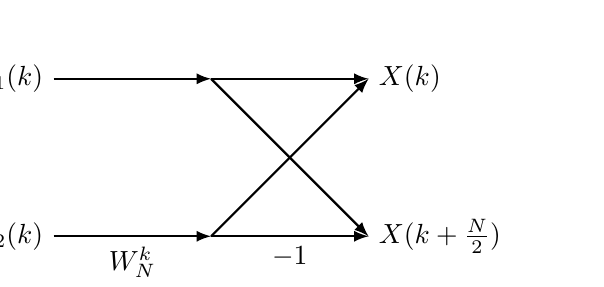
\begin{tikzpicture}
    \tikz[thick]{
    \draw[-latex] (2,1) -- (4,1);
    \draw[-latex] (4,1) -- (6,1);
    \draw[-latex] (2,3) -- (4,3);
    \draw[-latex] (4,3) -- (6,3);
    \draw[-latex] (4,1) -- (6,3);
    \draw[-latex] (4,3) -- (6,1);
    \node[left] at (2,1) {$X_2(k)$};
    \node[left] at (2,3) {$X_1(k)$};
    \node[below] at (3,1) {$W_N^k$};
    \node[below] at (5,1) {$-1$};
    \node[right] at (6,1) {$X(k+\frac{N}{2})$};
    \node[right] at (6,3) {$X(k)$};
    }
\end{tikzpicture}
\end{center}

每个蝶形运算有一次复乘,两次复加。$\dfrac{N}{2}$个蝶形运算的运算量:复乘$\dfrac{N}{2}$次;复加$N$次。总运算量:复乘$\dfrac{N^2}{2}+\dfrac{N}{2}\approx \dfrac{N^2}{2}$次;复加$\dfrac{N^2}{2}$次。

每个蝶形运算单元仅与蝶形的2个输入有关,这4个值均与其它蝶形运算无关,而且2个输入值在计算完输出值后没有其它用途。因此,可用2个输入单元保存2个输出值。即实现所谓原位运算。

\textbf{倒位序规律}

输出$X(k)$按正常顺序排列在存储单元,而输入是按顺序(0,4,2,6,1,5,3,7)。这种顺序称作倒位序,即下标写成二进制数再按位倒过来。

\begin{table}[htbp]
\centering
\begin{tabular}{|c|c|c|c|c|c|c|c|}
    $X(0)$ & $X(1)$ & $X(2)$ & $X(3)$ & $X(4)$ & $X(5)$ & $X(6)$ & $X(7)$ \\
    000 & 001 & 010 & 011 & 100 & 101 & 110 & 111 \\
    000 & 100 & 010 & 110 & 001 & 101 & 011 & 111 \\
    $x(0)$ & $x(4)$ & $x(2)$ & $x(6)$ & $x(1)$ & $x(5)$ & $x(3)$ & $x(7)$
\end{tabular}
\end{table}

倒位序在DSP中实现:

将AR0置$\dfrac{N}{2}$,输入序列基址存入ARx,倒位序寻址*ARx+0B,即ARx以倒位序进位的方式加上AR0。

\textbf{DIT运算流图}

以$N=8$点DFT为例,运算流图如下:

\begin{center}
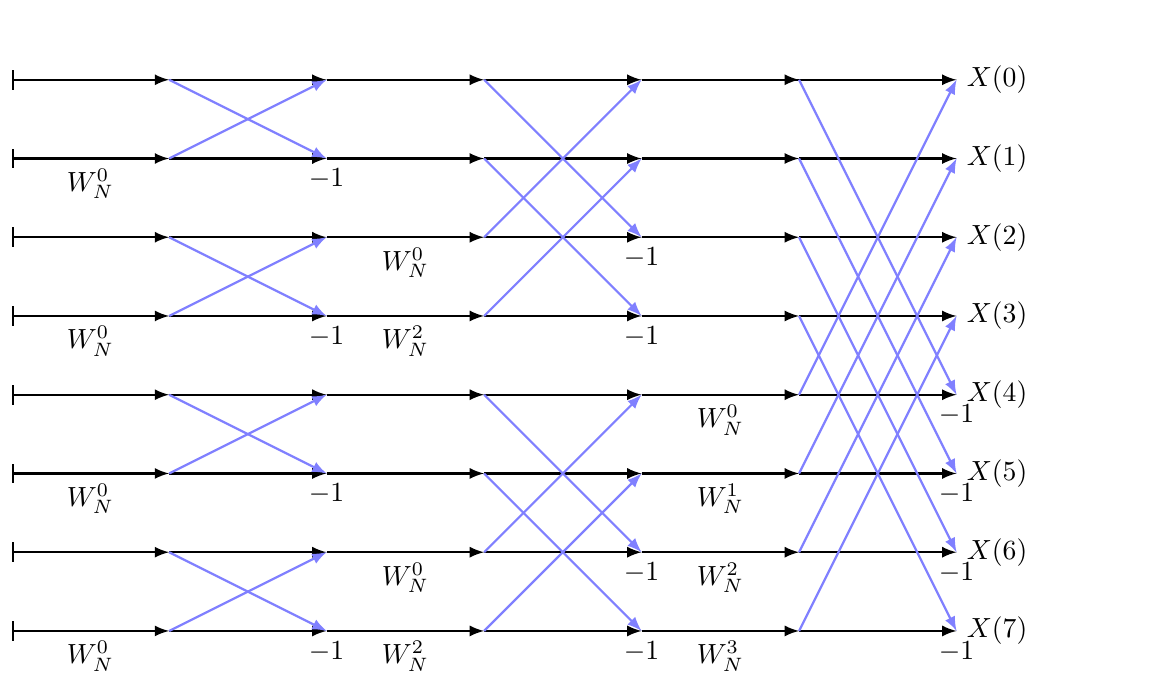
\begin{tikzpicture}[yscale=0.5]
    \tikz[thick]{
    \draw[|-latex] (2,1) -- (4,1);
    \draw[-latex] (4,1) -- (6,1);
    \draw[|-latex] (2,2) -- (4,2);
    \draw[-latex] (4,2) -- (6,2);
    \draw[|-latex] (2,3) -- (4,3);
    \draw[-latex] (4,3) -- (6,3);
    \draw[|-latex] (2,4) -- (4,4);
    \draw[-latex] (4,4) -- (6,4);
    \draw[|-latex] (2,5) -- (4,5);
    \draw[-latex] (4,5) -- (6,5);
    \draw[|-latex] (2,6) -- (4,6);
    \draw[-latex] (4,6) -- (6,6);
    \draw[|-latex] (2,7) -- (4,7);
    \draw[-latex] (4,7) -- (6,7);
    \draw[|-latex] (2,8) -- (4,8);
    \draw[-latex] (4,8) -- (6,8);%
    \draw[blue!50,-latex] (4,1) -- (6,2);
    \draw[blue!50,-latex] (4,2) -- (6,1);
    \draw[blue!50,-latex] (4,3) -- (6,4);
    \draw[blue!50,-latex] (4,4) -- (6,3);
    \draw[blue!50,-latex] (4,5) -- (6,6);
    \draw[blue!50,-latex] (4,6) -- (6,5);
    \draw[blue!50,-latex] (4,7) -- (6,8);
    \draw[blue!50,-latex] (4,8) -- (6,7);%
    \draw[-latex] (6,1) -- (8,1);
    \draw[-latex] (8,1) -- (10,1);
    \draw[-latex] (6,2) -- (8,2);
    \draw[-latex] (8,2) -- (10,2);
    \draw[-latex] (6,3) -- (8,3);
    \draw[-latex] (8,3) -- (10,3);
    \draw[-latex] (6,4) -- (8,4);
    \draw[-latex] (8,4) -- (10,4);
    \draw[-latex] (6,5) -- (8,5);
    \draw[-latex] (8,5) -- (10,5);
    \draw[-latex] (6,6) -- (8,6);
    \draw[-latex] (8,6) -- (10,6);
    \draw[-latex] (6,7) -- (8,7);
    \draw[-latex] (8,7) -- (10,7);
    \draw[-latex] (6,8) -- (8,8);
    \draw[-latex] (8,8) -- (10,8);%
    \draw[blue!50,-latex] (8,1) -- (10,3);
    \draw[blue!50,-latex] (8,2) -- (10,4);
    \draw[blue!50,-latex] (8,3) -- (10,1);
    \draw[blue!50,-latex] (8,4) -- (10,2);
    \draw[blue!50,-latex] (8,5) -- (10,7);
    \draw[blue!50,-latex] (8,6) -- (10,8);
    \draw[blue!50,-latex] (8,7) -- (10,5);
    \draw[blue!50,-latex] (8,8) -- (10,6);%
    \draw[-latex] (10,1) -- (12,1);
    \draw[-latex] (12,1) -- (14,1);
    \draw[-latex] (10,2) -- (12,2);
    \draw[-latex] (12,2) -- (14,2);
    \draw[-latex] (10,3) -- (12,3);
    \draw[-latex] (12,3) -- (14,3);
    \draw[-latex] (10,4) -- (12,4);
    \draw[-latex] (12,4) -- (14,4);
    \draw[-latex] (10,5) -- (12,5);
    \draw[-latex] (12,5) -- (14,5);
    \draw[-latex] (10,6) -- (12,6);
    \draw[-latex] (12,6) -- (14,6);
    \draw[-latex] (10,7) -- (12,7);
    \draw[-latex] (12,7) -- (14,7);
    \draw[-latex] (10,8) -- (12,8);
    \draw[-latex] (10,8) -- (14,8);%
    \draw[blue!50,-latex] (12,1) -- (14,5);
    \draw[blue!50,-latex] (12,2) -- (14,6);
    \draw[blue!50,-latex] (12,3) -- (14,7);
    \draw[blue!50,-latex] (12,4) -- (14,8);
    \draw[blue!50,-latex] (12,5) -- (14,1);
    \draw[blue!50,-latex] (12,6) -- (14,2);
    \draw[blue!50,-latex] (12,7) -- (14,3);
    \draw[blue!50,-latex] (12,8) -- (14,4);%
    \node[left] at (2,1) {$x(7)$};
    \node[left] at (2,2) {$x(3)$};
    \node[left] at (2,3) {$x(5)$};
    \node[left] at (2,4) {$x(1)$};
    \node[left] at (2,5) {$x(6)$};
    \node[left] at (2,6) {$x(2)$};
    \node[left] at (2,7) {$x(4)$};
    \node[left] at (2,8) {$x(0)$};%
    \node[right] at (14,1) {$X(7)$};
    \node[right] at (14,2) {$X(6)$};
    \node[right] at (14,3) {$X(5)$};
    \node[right] at (14,4) {$X(4)$};
    \node[right] at (14,5) {$X(3)$};
    \node[right] at (14,6) {$X(2)$};
    \node[right] at (14,7) {$X(1)$};
    \node[right] at (14,8) {$X(0)$};%
    \node[below] at (3,1) {$W_N^0$};
    \node[below] at (3,3) {$W_N^0$};
    \node[below] at (3,5) {$W_N^0$};
    \node[below] at (3,7) {$W_N^0$};%
    \node[below] at (6,1) {$-1$};
    \node[below] at (6,3) {$-1$};
    \node[below] at (6,5) {$-1$};
    \node[below] at (6,7) {$-1$};%
    \node[below] at (7,1) {$W_N^2$};
    \node[below] at (7,2) {$W_N^0$};
    \node[below] at (7,5) {$W_N^2$};
    \node[below] at (7,6) {$W_N^0$};%
    \node[below] at (10,1) {$-1$};
    \node[below] at (10,2) {$-1$};
    \node[below] at (10,5) {$-1$};
    \node[below] at (10,6) {$-1$};%
    \node[below] at (11,1) {$W_N^3$};
    \node[below] at (11,2) {$W_N^2$};
    \node[below] at (11,3) {$W_N^1$};
    \node[below] at (11,4) {$W_N^0$};%
    \node[below] at (14,1) {$-1$};
    \node[below] at (14,2) {$-1$};
    \node[below] at (14,3) {$-1$};
    \node[below] at (14,4) {$-1$};%
    }
\end{tikzpicture}
\end{center}

当$N=2^L$时共需$L$级蝶形运算,每往前一级,系数个数减半,系数指数乘2。第一级加权系数只有$W_N^0=1$,没有乘法;第二级系数为2个,$W_N^0=1, W_N^{\frac{N}{4}}=\text{j}$,也可以不用乘法计算;最后一级系数为$\frac{N}{2}$个。

\textbf{存储单元}

输入序列$x(n), 0\leq n\leq N-1$,共$N$个单元;加权系数$W_N^r, 0\leq r\leq \dfrac{N}{2}-1$,需$\dfrac{N}{2}$个存储单元;共计$\dfrac{3}{2}N$个存储单元。

\textbf{用FFT算法实现IFFT}

\begin{quote}
\begin{enumerate}
    \item 将$X(k)$取共轭。
    \item 对$X^*(k)$直接作FFT。
    \item 对FFT的结果取共轭并乘以$\dfrac{1}{N}$,得$x(n)$。
\end{enumerate}
\end{quote}

\textbf{用$N$点FFT运算计算$2N$点实序列的FFT}

\begin{quote}
\begin{enumerate}
    \item 将$x(n)$分为偶数组$x_1(n)$和奇数组$x_2(n)$。
    \item 将$x_1(n)$及$x_2(n)$组成一个复序列$y(n)=x_1(n)+\text{j}x_2(n)$。
    \item 通过$N$点FFT运算可得$Y(k)=X_1(k)+\text{j}X_2(k)$。
    \item $X(k)=X_1(k)+W_{2N}^{k}X_2(k)$。
\end{enumerate}
\end{quote}

\subsection{按频率抽取(DIF)的基-2 FFT算法}

\textbf{DIF蝶形运算}

\begin{equation}
\begin{array}{ll}
    x_1(n)=x(n)+x\left(n+\dfrac{N}{2}\right), & 0\leq n\leq \dfrac{N}{2}-1 \\
    x_2(n)=\left[x(n)-x\left(n+\dfrac{N}{2}\right)\right]W_N^n, & 0\leq n\leq \dfrac{N}{2}-1
\end{array}
\end{equation}

DIF蝶形运算的运算结构如下:

\begin{center}
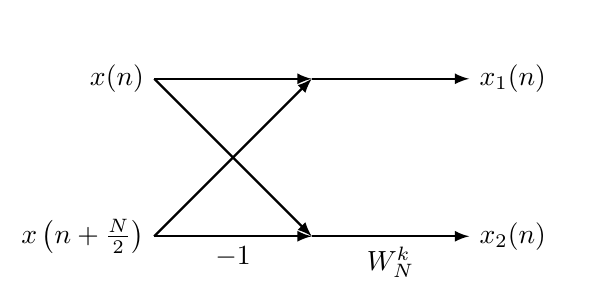
\begin{tikzpicture}
    \tikz[thick]{
    \draw[-latex] (2,1) -- (4,1);
    \draw[-latex] (4,1) -- (6,1);
    \draw[-latex] (2,3) -- (4,3);
    \draw[-latex] (4,3) -- (6,3);
    \draw[-latex] (2,1) -- (4,3);
    \draw[-latex] (2,3) -- (4,1);
    \node[left] at (2,1) {$x\left(n+\frac{N}{2}\right)$};
    \node[left] at (2,3) {$x(n)$};
    \node[below] at (5,1) {$W_N^k$};
    \node[below] at (3,1) {$-1$};
    \node[right] at (6,1) {$x_2(n)$};
    \node[right] at (6,3) {$x_1(n)$};
    }
\end{tikzpicture}
\end{center}

\textbf{DIF运算流图}

以$N=8$点DFT为例,运算流图如下:

\begin{center}
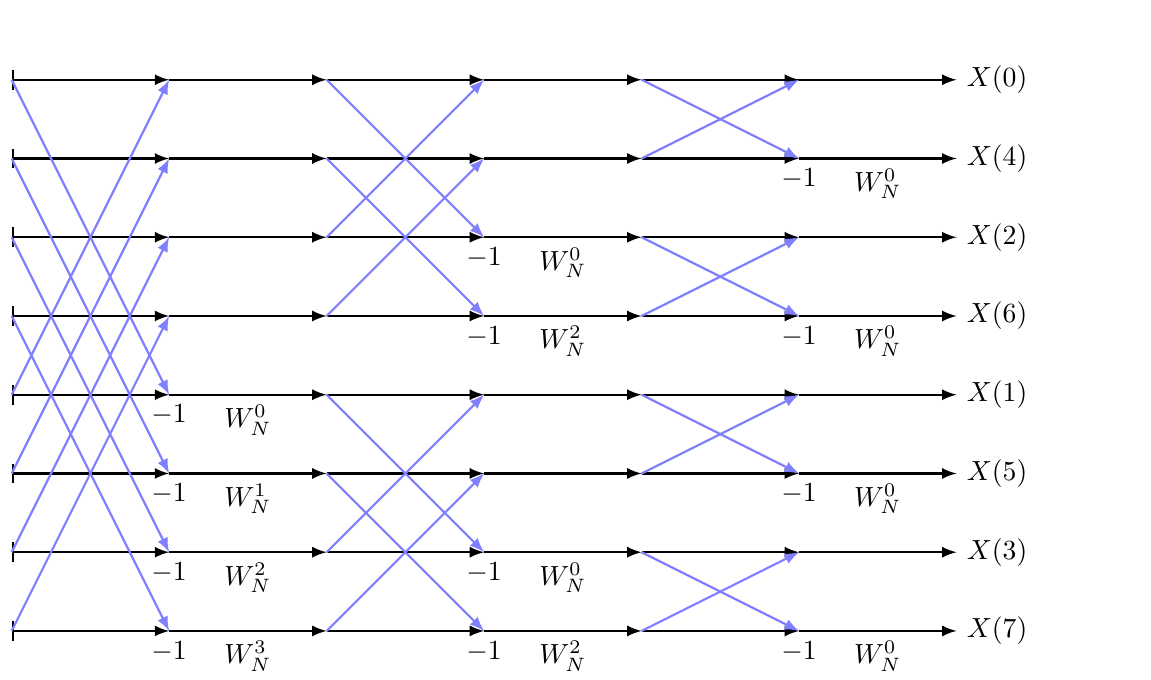
\begin{tikzpicture}[yscale=0.5]
    \tikz[thick]{
    \draw[|-latex] (2,1) -- (4,1);
    \draw[-latex] (4,1) -- (6,1);
    \draw[|-latex] (2,2) -- (4,2);
    \draw[-latex] (4,2) -- (6,2);
    \draw[|-latex] (2,3) -- (4,3);
    \draw[-latex] (4,3) -- (6,3);
    \draw[|-latex] (2,4) -- (4,4);
    \draw[-latex] (4,4) -- (6,4);
    \draw[|-latex] (2,5) -- (4,5);
    \draw[-latex] (4,5) -- (6,5);
    \draw[|-latex] (2,6) -- (4,6);
    \draw[-latex] (4,6) -- (6,6);
    \draw[|-latex] (2,7) -- (4,7);
    \draw[-latex] (4,7) -- (6,7);
    \draw[|-latex] (2,8) -- (4,8);
    \draw[-latex] (4,8) -- (6,8);%
    \draw[blue!50,-latex] (2,1) -- (4,5);
    \draw[blue!50,-latex] (2,2) -- (4,6);
    \draw[blue!50,-latex] (2,3) -- (4,7);
    \draw[blue!50,-latex] (2,4) -- (4,8);
    \draw[blue!50,-latex] (2,5) -- (4,1);
    \draw[blue!50,-latex] (2,6) -- (4,2);
    \draw[blue!50,-latex] (2,7) -- (4,3);
    \draw[blue!50,-latex] (2,8) -- (4,4);%
    \draw[-latex] (6,1) -- (8,1);
    \draw[-latex] (8,1) -- (10,1);
    \draw[-latex] (6,2) -- (8,2);
    \draw[-latex] (8,2) -- (10,2);
    \draw[-latex] (6,3) -- (8,3);
    \draw[-latex] (8,3) -- (10,3);
    \draw[-latex] (6,4) -- (8,4);
    \draw[-latex] (8,4) -- (10,4);
    \draw[-latex] (6,5) -- (8,5);
    \draw[-latex] (8,5) -- (10,5);
    \draw[-latex] (6,6) -- (8,6);
    \draw[-latex] (8,6) -- (10,6);
    \draw[-latex] (6,7) -- (8,7);
    \draw[-latex] (8,7) -- (10,7);
    \draw[-latex] (6,8) -- (8,8);
    \draw[-latex] (8,8) -- (10,8);%
    \draw[blue!50,-latex] (6,1) -- (8,3);
    \draw[blue!50,-latex] (6,2) -- (8,4);
    \draw[blue!50,-latex] (6,3) -- (8,1);
    \draw[blue!50,-latex] (6,4) -- (8,2);
    \draw[blue!50,-latex] (6,5) -- (8,7);
    \draw[blue!50,-latex] (6,6) -- (8,8);
    \draw[blue!50,-latex] (6,7) -- (8,5);
    \draw[blue!50,-latex] (6,8) -- (8,6);%
    \draw[-latex] (10,1) -- (12,1);
    \draw[-latex] (12,1) -- (14,1);
    \draw[-latex] (10,2) -- (12,2);
    \draw[-latex] (12,2) -- (14,2);
    \draw[-latex] (10,3) -- (12,3);
    \draw[-latex] (12,3) -- (14,3);
    \draw[-latex] (10,4) -- (12,4);
    \draw[-latex] (12,4) -- (14,4);
    \draw[-latex] (10,5) -- (12,5);
    \draw[-latex] (12,5) -- (14,5);
    \draw[-latex] (10,6) -- (12,6);
    \draw[-latex] (12,6) -- (14,6);
    \draw[-latex] (10,7) -- (12,7);
    \draw[-latex] (12,7) -- (14,7);
    \draw[-latex] (10,8) -- (12,8);
    \draw[-latex] (10,8) -- (14,8);%
    \draw[blue!50,-latex] (10,1) -- (12,2);
    \draw[blue!50,-latex] (10,2) -- (12,1);
    \draw[blue!50,-latex] (10,3) -- (12,4);
    \draw[blue!50,-latex] (10,4) -- (12,3);
    \draw[blue!50,-latex] (10,5) -- (12,6);
    \draw[blue!50,-latex] (10,6) -- (12,5);
    \draw[blue!50,-latex] (10,7) -- (12,8);
    \draw[blue!50,-latex] (10,8) -- (12,7);%
    \node[left] at (2,1) {$x(7)$};
    \node[left] at (2,2) {$x(6)$};
    \node[left] at (2,3) {$x(5)$};
    \node[left] at (2,4) {$x(4)$};
    \node[left] at (2,5) {$x(3)$};
    \node[left] at (2,6) {$x(2)$};
    \node[left] at (2,7) {$x(1)$};
    \node[left] at (2,8) {$x(0)$};%
    \node[right] at (14,1) {$X(7)$};
    \node[right] at (14,2) {$X(3)$};
    \node[right] at (14,3) {$X(5)$};
    \node[right] at (14,4) {$X(1)$};
    \node[right] at (14,5) {$X(6)$};
    \node[right] at (14,6) {$X(2)$};
    \node[right] at (14,7) {$X(4)$};
    \node[right] at (14,8) {$X(0)$};%
    \node[below] at (13,1) {$W_N^0$};
    \node[below] at (13,3) {$W_N^0$};
    \node[below] at (13,5) {$W_N^0$};
    \node[below] at (13,7) {$W_N^0$};%
    \node[below] at (12,1) {$-1$};
    \node[below] at (12,3) {$-1$};
    \node[below] at (12,5) {$-1$};
    \node[below] at (12,7) {$-1$};%
    \node[below] at (9,1) {$W_N^2$};
    \node[below] at (9,2) {$W_N^0$};
    \node[below] at (9,5) {$W_N^2$};
    \node[below] at (9,6) {$W_N^0$};%
    \node[below] at (8,1) {$-1$};
    \node[below] at (8,2) {$-1$};
    \node[below] at (8,5) {$-1$};
    \node[below] at (8,6) {$-1$};%
    \node[below] at (5,1) {$W_N^3$};
    \node[below] at (5,2) {$W_N^2$};
    \node[below] at (5,3) {$W_N^1$};
    \node[below] at (5,4) {$W_N^0$};%
    \node[below] at (4,1) {$-1$};
    \node[below] at (4,2) {$-1$};
    \node[below] at (4,3) {$-1$};
    \node[below] at (4,4) {$-1$};%
    }
\end{tikzpicture}
\end{center}

\textbf{DIT与DIF的异同}

\begin{quote}
\begin{enumerate}
    \item 均进行原位运算。
    \item 运算量相同。
    \item DIT输入倒位序,输出为自然顺序;DIF与此相反。
    \item 蝶形运算不同(互为转置)。
\end{enumerate}
\end{quote}

\subsection{线性卷积与线性相关的FFT算法}

\subsubsection{线性卷积的FFT算法}

\begin{quote}
\begin{enumerate}
    \item 将序列$x(n), h(n)$补零成$N$点序列,$N=2^r\geq N_x+N_h-1$。
    \item 计算$X(k)=\text{FFT}[x(n)], H(k)=\text{FFT}[h(n)]$,$N$点FFT变换。
    \item 求$Y(k)=X(k)\cdot H(k)$,$N$个复数乘法。
    \item 计算$y(n)=\text{IFFT}[Y(k)]$,$N$点IFFT变换。
\end{enumerate}
\end{quote}

只要进行二次FFT,一次IFFT就可完成线性卷积计算。当$x(n), h(n)$两序列长度接近或相等时,有以下结论($L=N_x=N_h$):

\begin{quote}
\begin{enumerate}
    \item $L=8, 16, 32$时,圆周卷积的运算量大于线性卷积。
    \item $L=64$时,圆周卷积和线性卷积运算量相当。
    \item $L>64$时,圆周卷积的运算量大于线性卷积。
\end{enumerate}
\end{quote}

因此称圆周卷积为快速卷积。

如果$x(n), h(n)$长度相差较大,为了保持快速卷积法的优越性,可将$x(n)$分为许多段,每段的长度与$h(n)$接近,有重叠相加法和重叠保留法两种处理方法。

\textbf{重叠相加法}

\begin{quote}
\begin{enumerate}
    \item 将序列$h(n)$补零成$N$点序列,$N=2^r\geq N_x+N_h-1$。
    \item 计算$X_i(k)=\text{FFT}[x_i(n)], H(k)=\text{FFT}[h(n)]$,$N$点FFT变换。
    \item 求$Y_i(k)=X_i(k)\cdot H(k)$,$N$个复数乘法。
    \item 计算$y_i(n)=\text{IFFT}[Y_i(k)]$,$N$点IFFT变换。
    \item 将重叠部分的$N_h-1$个值相加。
\end{enumerate}
\end{quote}

\textbf{重叠保留法}

和重叠相加法的区别:$x(n)$的分段序列中第一段补$N_h-1$个零,后面的分段补前一个分段的最后$N_h-1$个值。每段卷积结果中前$N_h-1$个点舍去。

\subsubsection{线性相关的FFT算法}

\begin{quote}
\begin{enumerate}
    \item 将序列$x(n), y(n)$补零成$N$点序列,$N=2^r\geq N_x+N_y-1$。
    \item 计算$X(k)=\text{FFT}[x(n)], Y(k)=\text{FFT}[y(n)]$,$N$点FFT变换。
    \item 求$R_{xy}(k)=X(k)\cdot Y^*(k)$,$N$个复数乘法。
    \item 计算$r_{xy}(n)=\text{IFFT}[R_{xy}(k)]$,$N$点IFFT变换。
\end{enumerate}
\end{quote}

\section{数字滤波器}

\subsection{滤波器}

滤波器是对波进行过滤的器件。

滤波器的差分方程表示为

\begin{equation}
    y(n)=\sum_{k=1}^{N}a_k y(n-k)+\sum_{k=0}^{M}b_k x(n-k)
\end{equation}

一个滤波系统的输出是其过去$N$点输出的线性组合加上当前输入序列与过去$M$点输入序列的线性组合。系统当前的输出与当前的输入、过去的输入和过去的输出有关,系统是带有记忆的。

滤波器的分类:

\begin{quote}
\begin{enumerate}
    \item 按所处理的信号:模拟滤波器和数字滤波器。
    \item 按所通过信号的频段:低通、高通、带通和带阻滤波器。
    \item 按所采用的元器件:无源和有源滤波器。
\end{enumerate}
\end{quote}

数字滤波器的实现方法:直接利用通用计算机和通用软件编程实现;
或利用专用数字硬件、专用的DSP芯片实现。

数字滤波的基本操作:加法、乘法、延迟。

\subsection{IIR滤波器}

\subsubsection{IIR滤波器的特点}

\begin{quote}
\begin{enumerate}
    \item 单位冲激响应$h(n)$是无限长的。
    \item 系统函数$H(z)$在有限$z$平面上有极点存在,系统可能不稳定。
    \item 结构上是递归型的,即存在着输出到输入的反馈。
\end{enumerate}
\end{quote}

\subsubsection{IIR滤波器的基本结构}

IIR滤波器系统函数为

\begin{equation}
    H(z)=\frac{Y(z)}{X(z)}=\frac{\sum\limits_{k=0}^{M}b_k z^{-k}}{1-\sum\limits_{k=1}^{N}a_k z^{-k}}
\end{equation}

\textbf{直接\uppercase\expandafter{\romannumeral1}型结构}

直接\uppercase\expandafter{\romannumeral1}型结构结构流图如下:

\begin{center}
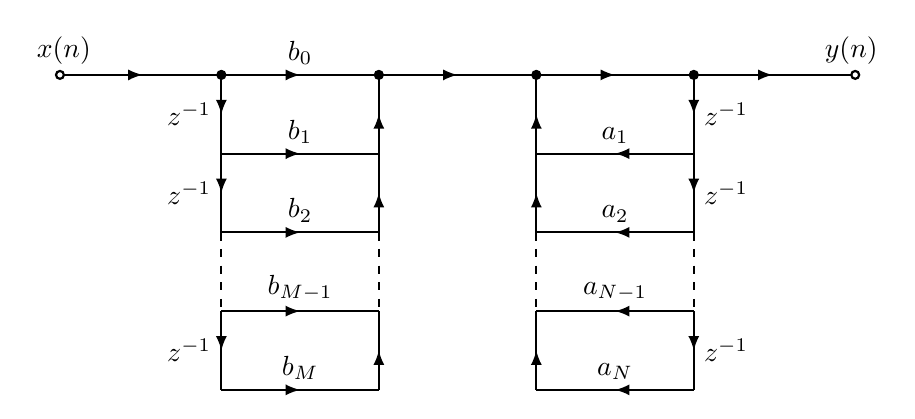
\begin{tikzpicture}[thick]
    \draw (1.95,5) circle [radius=0.05];
    \draw (12.05,5) circle [radius=0.05];
    \draw (2,5) -- (12,5);
    
    \filldraw (4,5) circle [radius=0.05];
    \filldraw (6,5) circle [radius=0.05];
    \filldraw (8,5) circle [radius=0.05];
    \filldraw (10,5) circle [radius=0.05];

    \draw[-latex] (2,5) -- (3,5);
    \draw[-latex] (4,5) -- (5,5);
    \draw[-latex] (6,5) -- (7,5);
    \draw[-latex] (8,5) -- (9,5);
    \draw[-latex] (10,5) -- (11,5);

    \foreach \i in {1,2,3,4}{
        \draw (4,\i) -- (6,\i);
        \draw[-latex] (4,\i) -- (5,\i);
        \draw (10,\i) -- (8,\i);
        \draw[-latex] (10,\i) -- (9,\i);
    }

    \foreach \i in {4,6,8,10}{
        \draw (\i,5) -- (\i,3);
        \draw[dashed] (\i,3) -- (\i,2);
        \draw (\i,2) -- (\i,1);
    }

    \foreach \i in {4,10}{
        \draw[-latex] (\i,5) -- (\i,4.5);
        \draw[-latex] (\i,4) -- (\i,3.5);
        \draw[-latex] (\i,2) -- (\i,1.5);
    }

    \foreach \i in {6,8}{
        \draw[-latex] (\i,4) -- (\i,4.5);
        \draw[-latex] (\i,3) -- (\i,3.5);
        \draw[-latex] (\i,1) -- (\i,1.5);
    }
    
    \node[above] at (2,5) {$x(n)$};
    \node[above] at (12,5) {$y(n)$};

    \foreach \i in {1.5,3.5,4.5}{
        \node[left] at (4,\i) {$z^{-1}$};
        \node[right] at (10,\i) {$z^{-1}$};
    }

    \node[above] at (5,5) {$b_0$};
    \node[above] at (5,4) {$b_1$};
    \node[above] at (5,3) {$b_2$};
    \node[above] at (5,2) {$b_{M-1}$};
    \node[above] at (5,1) {$b_M$};

    \node[above] at (9,4) {$a_1$};
    \node[above] at (9,3) {$a_2$};
    \node[above] at (9,2) {$a_{N-1}$};
    \node[above] at (9,1) {$a_N$};

\end{tikzpicture}
\end{center}

\textbf{直接\uppercase\expandafter{\romannumeral2}型(典范型)结构}

直接\uppercase\expandafter{\romannumeral2}型结构结构流图如下:

\begin{center}
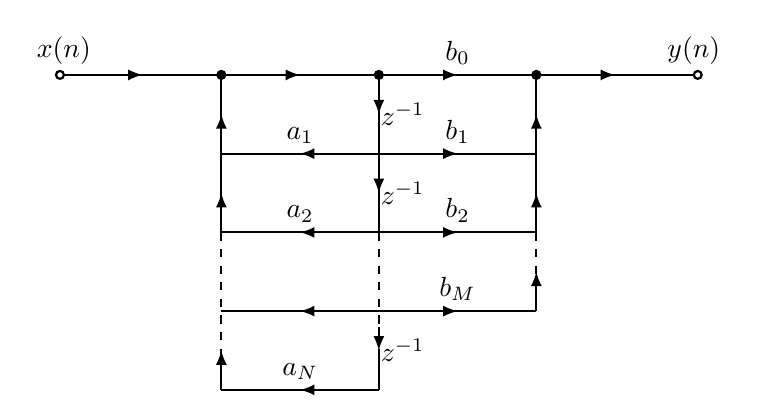
\begin{tikzpicture}[thick]
    \draw (1.95,5) circle [radius=0.05];
    \draw (10.05,5) circle [radius=0.05];
    \draw (2,5) -- (10,5);
    
    \filldraw (4,5) circle [radius=0.05];
    \filldraw (6,5) circle [radius=0.05];
    \filldraw (8,5) circle [radius=0.05];

    \draw[-latex] (2,5) -- (3,5);
    \draw[-latex] (4,5) -- (5,5);
    \draw[-latex] (6,5) -- (7,5);
    \draw[-latex] (8,5) -- (9,5);

    \foreach \i in {1,2,3,4}{
        \draw (4,\i) -- (6,\i);
        \draw[-latex] (6,\i) -- (5,\i);
    }

    \foreach \i in {2,3,4}{
        \draw (8,\i) -- (6,\i);
        \draw[-latex] (6,\i) -- (7,\i);
    }

    \foreach \i in {4,6}{
        \draw (\i,5) -- (\i,3);
        \draw[dashed] (\i,3) -- (\i,1.5);
        \draw (\i,1.5) -- (\i,1);
    }

    \foreach \i in {4,6,8}{
        \draw (\i,5) -- (\i,3);
        \draw[dashed] (\i,3) -- (\i,2);
    }

    \foreach \i in {6}{
        \draw[-latex] (\i,5) -- (\i,4.5);
        \draw[-latex] (\i,4) -- (\i,3.5);
        \draw[-latex] (\i,1.8) -- (\i,1.5);
    }

    \foreach \i in {4}{
        \draw[-latex] (\i,4) -- (\i,4.5);
        \draw[-latex] (\i,3) -- (\i,3.5);
        \draw[-latex] (\i,1) -- (\i,1.5);
    }

    \foreach \i in {8}{
        \draw[-latex] (\i,4) -- (\i,4.5);
        \draw[-latex] (\i,3) -- (\i,3.5);
        \draw[-latex] (\i,2) -- (\i,2.5);
    }
    
    \node[above] at (2,5) {$x(n)$};
    \node[above] at (10,5) {$y(n)$};

    \foreach \i in {1.5,3.5,4.5}{
        \node[right=-3pt] at (6,\i) {$z^{-1}$};
    }

    \node[above] at (7,5) {$b_0$};
    \node[above] at (7,4) {$b_1$};
    \node[above] at (7,3) {$b_2$};
    \node[above] at (7,2) {$b_M$};

    \node[above] at (5,4) {$a_1$};
    \node[above] at (5,3) {$a_2$};
    \node[above] at (5,1) {$a_N$};

\end{tikzpicture}
\end{center}

\textbf{级联型结构}

把$H(z)$分解成几个一阶或二阶数字网络的级联形式

\begin{equation}
    H(z)=A\prod_{i=1}^{K}H_i(z)
\end{equation}

\textbf{并联型结构}

把$H(z)$分解成几个一阶或二阶数字网络的并联形式

\begin{equation}
    H(z)=\sum_{i=1}^{K}H_i(z)
\end{equation}

\subsubsection{转置定理}

如果将原网络中所有支路方向加以倒转,且将输入和输出交换,其系统函数仍不改变。

\subsection{FIR滤波器}

\subsubsection{FIR滤波器的特点}

\begin{quote}
\begin{enumerate}
    \item 单位冲激响应$h(n)$是有限个非零值。
    \item $H(z)$在$|z|>0$处收敛,在$|z|>0$处只有零点,全部极点都在$z=0$处,因而系统总是因果稳定的。
    \item 结构上主要是非递归结构,没有输出到输入的反馈。
\end{enumerate}
\end{quote}

\subsubsection{FIR滤波器的基本结构}

FIR滤波器差分方程为

\begin{equation}
    y(n)=\sum_{m=0}^{N-1}h(m)x(n-m)
\end{equation}

\textbf{横截型(卷积型、直接型)结构}

横截型结构结构流图如下:

\begin{center}
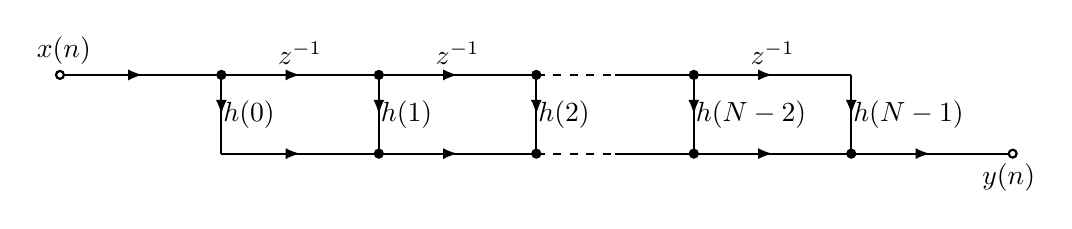
\begin{tikzpicture}[thick]
    \draw (1.95,2) circle [radius=0.05];
    \draw (2,2) -- (8,2);
    \draw[dashed] (8,2) -- (9,2);
    \draw (9,2) -- (12,2);

    \draw (14.05,1) circle [radius=0.05];
    \draw (4,1) -- (8,1);
    \draw[dashed] (8,1) -- (9,1);
    \draw (9,1) -- (14,1);

    \draw[-latex] (2,2) -- (3,2);
    \draw[-latex] (4,2) -- (5,2);
    \draw[-latex] (6,2) -- (7,2);
    \draw[-latex] (10,2) -- (11,2);
    \draw[-latex] (4,1) -- (5,1);
    \draw[-latex] (6,1) -- (7,1);
    \draw[-latex] (10,1) -- (11,1);
    \draw[-latex] (12,1) -- (13,1);

    \foreach \i in {4,6,8,10,12}{
        \draw (\i,1) -- (\i,2);
        \draw[-latex] (\i,2) -- (\i,1.5);
    }

    \foreach \i in {4,6,8,10}{
        \filldraw (\i,2) circle [radius=0.05];
    }

    \foreach \i in {6,8,10,12}{
        \filldraw (\i,1) circle [radius=0.05];
    }
    
    \node[above] at (2,2) {$x(n)$};
    \node[below] at (14,1) {$y(n)$};

    \foreach \i in {5,7,11}{
        \node[above] at (\i,2) {$z^{-1}$};
    }

    \node[right=-3pt] at (4,1.5) {$h(0)$};
    \node[right=-3pt] at (6,1.5) {$h(1)$};
    \node[right=-3pt] at (8,1.5) {$h(2)$};
    \node[right=-3pt] at (10,1.5) {$h(N-2)$};
    \node[right=-3pt] at (12,1.5) {$h(N-1)$};
\end{tikzpicture}
\end{center}

用转置定理可得另一种横截型结构。

\textbf{级联型结构}

把$H(z)$分解为实系数二阶因子的乘积形式

\begin{equation}
    H(z)=\prod_{k=0}^{\left\lceil\frac{N}{2}\right\rceil}(\beta_{0k}+\beta_{1k}z^{-1}+\beta_{2k}z^{-2})
\end{equation}
 
其中$\left\lceil\dfrac{N}{2}\right\rceil$表示对$\dfrac{N}{2}$向下取整。可以有一个$\beta_{2k}=0$,即得到一个一阶级联基本节。

级联型结构流图如下:

\begin{center}
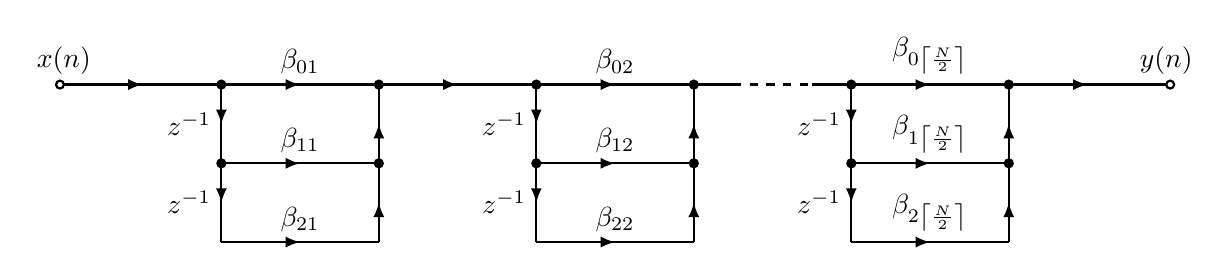
\begin{tikzpicture}[thick]
    \draw (1.95,3) circle [radius=0.05];
    \draw (16.05,3) circle [radius=0.05];
    \draw (2,3) -- (10.5,3);
    \draw[dashed] (10.5,3) -- (11.5,3);
    \draw (11.5,3) -- (16,3);

    \draw[-latex] (2,3) -- (3,3);
    \draw[-latex] (4,3) -- (5,3);
    \draw[-latex] (6,3) -- (7,3);
    \draw[-latex] (8,3) -- (9,3);
    \draw[-latex] (12,3) -- (13,3);
    \draw[-latex] (14,3) -- (15,3);

    \foreach \i in {4,6,8,10,12,14}{
        \filldraw (\i,3) circle [radius=0.05];
    }

    \foreach \i in {4,8,12}{
        \draw (\i,1) -- (\i,3);
        \filldraw (\i,2) circle [radius=0.05];
        \draw[-latex] (\i,3) -- (\i,2.5);
        \draw[-latex] (\i,2) -- (\i,1.5);
    }

    \foreach \i in {6,10,14}{
        \draw (\i,1) -- (\i,3);
        \filldraw (\i,2) circle [radius=0.05];
        \draw[-latex] (\i,2) -- (\i,2.5);
        \draw[-latex] (\i,1) -- (\i,1.5);
    }

    \draw (4,1) -- (6,1);
    \draw (4,2) -- (6,2);
    \draw (8,1) -- (10,1);
    \draw (8,2) -- (10,2);
    \draw (12,1) -- (14,1);
    \draw (12,2) -- (14,2);

    \draw[-latex] (4,1) -- (5,1);
    \draw[-latex] (4,2) -- (5,2);
    \draw[-latex] (8,1) -- (9,1);
    \draw[-latex] (8,2) -- (9,2);
    \draw[-latex] (12,1) -- (13,1);
    \draw[-latex] (12,2) -- (13,2);

    \node[above] at (2,3) {$x(n)$};
    \node[above] at (16,3) {$y(n)$};

    \node[above] at (5,3) {$\beta_{01}$};
    \node[above] at (5,2) {$\beta_{11}$};
    \node[above] at (5,1) {$\beta_{21}$};
    \node[above] at (9,3) {$\beta_{02}$};
    \node[above] at (9,2) {$\beta_{12}$};
    \node[above] at (9,1) {$\beta_{22}$};
    \node[above] at (13,3) {$\beta_{0\left\lceil\frac{N}{2}\right\rceil}$};
    \node[above] at (13,2) {$\beta_{1\left\lceil\frac{N}{2}\right\rceil}$};
    \node[above] at (13,1) {$\beta_{2\left\lceil\frac{N}{2}\right\rceil}$};

    \foreach \i in {4,8,12}{
        \node[left] at (\i,2.5) {$z^{-1}$};
        \node[left] at (\i,1.5) {$z^{-1}$};
    }
\end{tikzpicture}
\end{center}

\section{IIR滤波器的设计}

低通滤波器(LPF)通过变换可以得到其他几种滤波器:

\begin{quote}
\begin{enumerate}
    \item 高通滤波器(HPF):全通减低通。
    \item 带通滤波器(BPF):低通后高通。
    \item 带阻滤波器(BRF):低通加高通。
\end{enumerate}
\end{quote}

理想滤波器不可实现,只能以实际滤波器逼近。

\subsection{滤波器的性能指标}

\textbf{带宽}:当幅度降低到0.707时的宽度称为滤波器的带宽(3dB带宽)。

\textbf{通带、阻带与过渡带}:信号允许通过的频带为通带,完全不允许通过的频带为阻带,通带与阻带之间为过渡带。

\textbf{滚降与滚降率}:滤波器幅频特性在过渡带的衰减和衰减速度称为滚降与滚降率。

\textbf{阻带衰减}:输入信号在阻带的衰减量。

\textbf{带内平坦度}:通带和阻带内的平坦程度。

\subsection{IIR数字滤波器的设计方法}

用一因果稳定的离散LSI系统逼近给定的性能要求:

$$H(z)=\frac{\sum\limits_{k=0}^{M}b_k z^{-k}}{1-\sum\limits_{k=1}^{N}a_k z^{-k}}$$

$s$平面逼近为模拟滤波器;$z$平面逼近为数字滤波器。

\subsection{用模拟滤波器设计IIR数字滤波器}

\subsubsection{冲激响应不变法}

\begin{equation}
    H_a(s)=\sum_{k=1}^{N}\frac{A_k}{s-s_k} \Rightarrow H(z)=\sum_{k=1}^{N}\frac{A_k T}{1-\text{e}^{s_k T}z^{-1}} 
\end{equation}

其频率响应为

\begin{equation}
    H(\text{e}^{\text{j}\omega})\approx H_a\left(\text{j}\frac{\omega}{T}\right), |\omega|<\pi
\end{equation}

\textbf{冲激响应不变法的优缺点}

时域逼近良好、保持线性关系;产生频率响应混叠失真,只适用于限带模拟滤波器,低通、带通滤波器。

\subsubsection{双线性变换法}

\begin{equation}
    \begin{array}{cc}
    H(z)=H_a\left(c\dfrac{1-z^{-1}}{1+z^{-1}}\right)\\
    s=c\dfrac{1-z^{-1}}{1+z^{-1}}, \quad z=\dfrac{c+s}{c-s}, \quad \Omega=c\cdot\tan\dfrac{\Omega_1 T}{2}
    \end{array}
\end{equation}

变换常数$c$的选择:

\begin{quote}
\begin{enumerate}
    \item 低频处有较确切的对应关系:$c=\dfrac{2}{T}$。
    \item 要求$\Omega_c$和$\omega_c$严格相对应:$c=\Omega_c\cot\dfrac{\omega_c}{2}$。
\end{enumerate}
\end{quote}

\textbf{双线性变换法的优缺点}

避免了频率响应的混叠现象;但除了零频率附近,$\Omega$和$\omega$之间严重非线性,要求模拟滤波器的幅频响应为分段常数型,不然会产生畸变。

\subsection{常用模拟低通滤波器}

由幅度平方函数$|H_a(\text{j}\Omega)|^2$确定模拟滤波器的系统函数$H_a(s)$:

\begin{equation}
    |H_a(\text{j}\Omega)|^2=H_a(s)H_a(-s)|_{s=\text{j}\Omega}
\end{equation}

将左半平面的的极点归$H_a(s)$;以虚轴为对称轴的对称零点的任一半作为$H_a(s)$的零点,虚轴上的零点一半归$H_a(s)$。

\begin{quote}
\begin{enumerate}
    \item 由幅度平方函数得象限对称的$s$平面函数。
    \item 对比$H_a(\text{j}\Omega)$和$H_a(s)$,确定增益常数。
    \item 由零极点及增益常数,得$H_a(s)$。
\end{enumerate}
\end{quote}

\subsubsection{Butterworth滤波器}

Butterworth滤波器的幅度平方响应为

\begin{equation}
    |H_a(\text{j}\Omega)|^2=\frac{1}{1+\left(\dfrac{\Omega}{\Omega_c}\right)^{2N}}
\end{equation}

其中$N$为滤波器的阶数;$\Omega_c$为通带截止频率,即低通滤波器的3dB带宽。

Butterworth滤波器是一个全极点滤波器,极点在$s$平面呈象限对称,分布在Buttterworth圆上,共$2N$点。

\subsubsection{Chebyshev滤波器}

Chebyshev \uppercase\expandafter{\romannumeral1}型滤波器的幅度平方响应为

\begin{equation}
    |H_a(\text{j}\Omega)|^2=\frac{1}{1+\varepsilon^2 C_N^2 \left(\dfrac{\Omega}{\Omega_c}\right)}
\end{equation}

其中$N$为滤波器的阶数;$\Omega_c$为通带截止频率,不一定是3dB带宽;$C_N(x)$为$N$阶Chebyshev多项式。

$\varepsilon$表示通带波纹参数,$0<\varepsilon<1$,$\varepsilon$越大,波纹越大。

\subsubsection{Ellipse滤波器}

带内均匀波动、最快的滚降。

\subsubsection{Bessel滤波器}

最大相位平坦特性。

\section{FIR数字滤波器的设计}

\subsection{线性相位FIR数字滤波器的特性}

\subsubsection{FIR数字滤波器的特性}

FIR数字滤波器具有如下特性:

\begin{quote}
\begin{enumerate}
    \item 可得到严格的线性相位,又可具有任意的幅度特性。 
    \item 系统无反馈,是无条件稳定系统。
    \item 经过延迟,非因果系统可用因果系统实现。
    \item 滤波器的阶次较高。
\end{enumerate}
\end{quote}

\subsubsection{线性相位充分条件}

\textbf{第一类线性相位}

第一类线性相位条件满足

\begin{equation}
    \theta(\omega)=-\omega\tau
\end{equation}

群延时为$\tau$的第一类严格线性相位因果系统的充分条件为

\begin{equation}
    \left\{
    \begin{array}{l}
        h(n)=h(N-1-n), \quad 0\leq n\leq N-1 \\
        \tau=\dfrac{N-1}{2}
    \end{array}
    \right.
\end{equation}

\textbf{第二类线性相位}

第二类线性相位条件满足

\begin{equation}
    \theta(\omega)=-\omega\tau+\beta
\end{equation}

群延时为$\tau$的第二类线性相位因果系统的充分条件为

\begin{equation}
    \left\{
    \begin{array}{l}
        h(n)=h(N-1-n), \quad 0\leq n\leq N-1 \\
        \beta=\pm\dfrac{\pi}{2} \\
        \tau=\dfrac{N-1}{2}
    \end{array}
    \right.
\end{equation}

第二类线性相位因果系统除了具有严格的线性相位外,还有$90^{\circ}$的相移,因而又称为线性相位正交变换器。

\subsection{FIR滤波器设计法原理}

一般先给出为理想频率响应,现要求设计一个N点的FIR滤波器去逼近。设计方法有三种:窗函数设计法(时域)、频率采样法(频域)、最优化设计(频域等波纹)。

\subsection{窗函数设计法}

窗函数设计法的步骤:

\begin{quote}
\begin{enumerate}
    \item $H_d(\text{e}^{\text{j}\omega})\Rightarrow h_d(n)$。
    \item 求加窗截断后的序列$h(n)=h_d(n)w(n)$。
    \item 检验$H(\text{e}^{\text{j}\omega})=H_d(\text{e}^{\text{j}\omega})\ast W(\text{e}^{\text{j}\omega})$是否满足要求。
    \item 若不满足,则更改窗形状或者改变窗长点数重新设计。
\end{enumerate}
\end{quote}

各种窗函数的基本参数如表3示。

\begin{table}[htbp]
\centering
\caption{常用窗函数的基本参数}
\begin{tabular}{c|c|c|c|c}
    \toprule
    \multirow{2}*{\textbf{窗函数}} & \textbf{旁瓣峰值} & \textbf{主瓣宽度} & \textbf{过渡带宽} & \textbf{阻带最小衰减} \\
    ~ & (dB) & ($2\pi/N$) & ($2\pi/N$) & (dB) \\
    \midrule
    矩形窗 & $-13$ & $2$ & $0.9$ & $-21$ \\
    \hline
    三角形窗 & $-25$ & $4$ & $3.05$ & $-25$ \\
    \hline
    Hanning窗 & $-31$ & $4$ & $3.1$ & $-44$ \\
    \hline
    Hamming窗 & $-41$ & $4$ & $3.3$ & $-53$ \\
    \hline
    Blackman窗 & $-57$ & $6$ & $5.5$ & $-74$ \\
    \bottomrule
\end{tabular}
\end{table}

\subsubsection{矩形窗}

\begin{equation}
    w_R(n)=R_N(n), \quad W_R(\text{e}^{\text{j}\omega})=\frac{\sin\frac{\omega N}{2}}{\sin\frac{\omega}{2}}\text{e}^{-\text{j}\omega\frac{N-1}{2}}
\end{equation}

对频率响应起作用的是它的幅度函数$W_R(\omega)=\frac{\sin\frac{\omega N}{2}}{\sin\frac{\omega}{2}}$,线性相位部分$\text{e}^{-\text{j}\omega\frac{N-1}{2}}$则是表示延时一半长度。

窗函数的频率特性使矩形频率响应产生带内和带外波动。在在过渡带的两侧波动最大,约为8.95\%,与$N$无关,称为吉布斯效应。

过渡带宽等于窗函数频率响应的主瓣宽度。增大$N$,只能改变窗谱的主瓣宽度,不能改变主瓣与旁瓣的相对比例。

\subsubsection{三角形窗(Bartlett窗)}

\begin{equation}
    w(n)=\left\{
    \begin{array}{ll}
        \dfrac{2n}{N-1}, & 0 \leq n \leq \dfrac{N-1}{2} \\
        2-\dfrac{2n}{N-1}, & \dfrac{N-1}{2} \leq n \leq N-1
    \end{array}
    \right.
\end{equation}

\subsubsection{Hanning窗(升余弦窗)}

\begin{equation}
    w(n)=\frac{1}{2}\left[1-\cos\left(\frac{2\pi n}{N-1}\right)\right]R_N(n)
\end{equation}

\subsubsection{Hamming窗(改进的升余弦窗)}

\begin{equation}
    w(n)=\left[0.54-0.46\cos\left(\frac{2\pi n}{N-1}\right)\right]R_N(n)
\end{equation}

\subsubsection{Blackman窗(二阶升余弦窗)}

\begin{equation}
    w(n)=\left[0.42-0.5\cos\left(\frac{2\pi n}{N-1}\right)+0.08\cos\left(\frac{4\pi n}{N-1}\right)\right]R_N(n)
\end{equation}

\subsection{频率抽样设计法}

\subsubsection{设计方法}

对理想频率响应等间隔抽样,作为实际FIR数字滤波器的频率特性的抽样值。

\begin{equation}
    H(k)=H_d(k)=\left.H_d\left(\text{e}^{\text{j}\omega}\right)\right|_{\omega=\frac{2\pi}{N}k},\quad 0\leq k\leq N-1
\end{equation}

内插公式:

\begin{equation}
\begin{array}{c}
    H(z)=\dfrac{1-z^{-N}}{N}\sum\limits_{k=0}^{N-1}{\dfrac{H(k)}{1-W_{N}^{-k}z^{-1}}} \\
    \addlinespace
    H\left(\text{e}^{\text{j}\omega}\right)=\sum\limits_{k=0}^{N-1}{H(k)\varPhi\left(\omega-\dfrac{2\pi}{N}k\right)}, \quad 
    \varPhi(\omega)=\dfrac{1}{N}\dfrac{\sin\frac{N\omega}{2}}{\sin\frac{\omega}{2}} \text{e}^{-\text{j}\left(\frac{N-1}{2}\right)\omega}
\end{array}
\end{equation}

抽样点上,频率响应严格相等;抽样点之间,加权内插函数的延伸叠加;变化越平缓,内插越接近理想值,逼近误差较小。

\subsubsection{两种频率抽样}

对$H_d\left(\text{e}^{\text{j}\omega}\right)$进行频率抽样,就是在$z$平面单位圆上的$N$个等间隔点上抽取出频率响应值。按第一个抽样点的值可以分为两种抽样方式:第一种方式在$\omega=0$处,第二种方式在$\omega=\dfrac{\pi}{N}$处。每种方式又可分为$N$是偶数与$N$是奇数两种。

\subsubsection{过渡带抽样的优化设计}

增加过渡带抽样点,可加大阻带衰减,但导致过渡带变宽。

增加$N$,使抽样点变密,减小过渡带宽度,但会增加计算量。

\end{document}
